%%=============================================================================
%% Methodologie
%%=============================================================================
\chapter{\IfLanguageName{dutch}{Methodologie}{Methodology}}%
\label{ch:methodologie}

De eerste fase zal gewijd worden aan het analyseren van de concrete problemen die zich mogelijks kunnen voordoen bij het behouden van de originele firewall, dit kan gaan over technische en non-technische aspecten die mogelijks de dienstverlening binnen de productie kunnen verstoren en de financiële schade die VPK daar mogelijk zou kunnen door oplopen. Ook zal er worden gekeken hoe het implementeren van die nieuwe firewall toepassing dit probleem zouden kunnen beheren en voorkomen. Hiervoor zal er gebruik gemaakt worden van bedrijfsinterne knowledge bases, diverse papers en studies met betrekking tot netwerkbeveiliging. Zo zal er een beter inzicht te verkrijgen zijn over de mogelijke firewall opstellingen en welke strategieën er kunnen worden toegepast voor het beschermen van het ICS met behulp van firewalltoepassingen. Ook zal er worden gekeken naar andere aspecten die mogelijks spelen bij het maken van een doordachte keuze. Dit kan gaan over de ervaringen van het huidige netwerkteam met een bepaalde vendor. Maar mogelijks over de integratie met andere netwerkcomponenten en de mogelijkheid om de firewall centraal te beheren. De geschatte duurtijd van deze fase bedraagt drie dagen die verspreid zullen zijn over drie weken.

Tijdens de tweede fase zal er een interne bevraging zijn bij systeembeheerders en netwerkprofessionals op bedrijfsniveau. Hun jarenlange ervaring omtrent netwerkbeveiliging en het optimaliseren van talloze beveiligingsmaatregelen binnen VPK kan kostbare inzichten opleveren voor het achterhalen van de huidige netwerkopstelling van het bedrijf. Deze informatie zal gebruikt kunnen worden voor het configureren van de firewall zodanig dat deze optimaal geconfigureerd is in het netwerk. Zo kunnen we de schade die een aanval zou kunnen aanrichten zo minimaal mogelijk houden en zal de aanval de dienstverlening zo weinig mogelijk verstoren. Ook kan deze informatie nuttig zijn voor de evaluatie in de vijfde fase. De geschatte duurtijd van deze fase bedraagt drie dagen die verspreid zullen zijn over drie weken.

In de derde fase verwerken we de grote hoeveelheid verzamelde data om een helder overzicht te creëren. Dit maakt het makkelijker om te beslissen of we de huidige firewall opnieuw configureren of een volledig nieuwe implementeren. Deze keuze baseren we op verschillende analyses, zoals een SWOT en RASCI analyse. Hiermee brengen we niet alleen de technische voor- en nadelen in kaart, maar kijken we ook naar welke stakeholders welke taken op zich nemen na de implementatie. Op basis van deze inzichten stellen we een concreet plan op voor eventuele aanpassingen aan de firewall en het netwerk van de productiesite. De geschatte duurtijd van deze fase bedraagt twee dagen die verspreid zullen zijn over twee weken.

In het vierde deel zal er worden toegespitst op het perfectioneren van beveiligingstoepassingen. Hierbij zal er met behulp van het plan dat is opgesteld in de derde fase de huidige firewalltoepassing geherconfigureerd worden. Als er aan de hand van de verschillende analyses blijkt dat een andere firewall dan de huidige firewall een betere 'fit' zou kunnen zijn voor de eisen en noden van VPK, dan kan er worden gekozen om gebruik te maken van een compleet nieuwe firewall die ook betere bescherming zal bieden tegen aanvallen op het ICS. Ook zullen er aanpassingen kunnen worden aangebracht aan de rest van het netwerk die de firewall zou kunnen helpen bij het tegenhouden van aanvallen op het ICS. De geschatte duurtijd van deze fase bedraagt drie dagen die verspreid zullen zijn over drie weken.

De vijfde en tevens laatste fase zal bestaan uit het evalueren van de impact van de geherconfigureerde firewall en de voorgestelde aanpassingen aan het netwerk. Er zullen een reeks criteria worden opgesteld waaraan voldaan moet zijn. Deze criteria zullen er voor zorgen dat we duidelijk kunnen aantonen dat mogelijke wijzigingen die we hebben aangebracht het makkelijker maken voor de systeembeheerders om ook de firewall te beheren en ze ook een duidelijker inzicht krijgen van welke zaken er juist gebeuren aan de interne kant van de firewall. Daarnaast zal worden beschreven welke specifieke maatregelen het beste kunnen worden genomen om het netwerk en de firewall van het productiebedrijf beter te beschermen tegen aanvallen op het ICS. De geschatte duur van deze fase bedraagt twee dagen, verdeeld over twee weken.  

\chapter{Analyse van het FR16 netwerk}

\label{ch:onderzoek}

\section{Analyse van de huidige opstelling}

De eerste fase van dit onderzoek richt zich voornamelijk op het verzamelen van relevante informatie die nodig is voor een weloverwogen keuze van de toekomstige firewallopstelling. Bij de implementatie van IT- of OT-toepassingen binnen een productiesite moet met een groot aantal factoren rekening worden gehouden. De hoogste prioriteit van elke productiesite blijft de continuïteit van de productie. Omdat de implementatie van een nieuwe netwerktopologie verschillende risico’s met zich meebrengt, is het cruciaal om alle mogelijke problemen en scenario’s zorgvuldig in kaart te brengen. Dit voorkomt verstoringen in het productieproces en waarborgt de continuiteit van de productie.
Een verstoring van de IT-dienstverlening binnen een productiesite heeft niet alleen impact op de IT-apparaten van gebruikers, maar ook op de OT toepassingen, zoals PLC’s, sensoren en SCADA-systemen. Deze systemen spelen een belangerijke rol in het aansturen en monitoren van industriële processen. Wanneer de IT infrastructuur faalt, kunnen deze OT systemen niet meer correct functioneren, dit heeft directe gevolgen voor de productieomgeving. Daarnaast is de werking van machines binnen een productiesite sterk afhankelijk van onderlinge communicatie tussen hen. Ze zijn geprogrammeerd om in een nauwkeurige volgorde en met optimale efficiëntie te opereren, zodat de productie soepel verloopt en de supply chain niet wordt onderbroken. Als de verbinding tussen deze machines wegvalt, ontstaan er onvoorziene stilstanden en inefficiënties die de productie ernstig kunnen vertragen of zelfs volledig stilleggen. Dit heeft niet alleen gevolgen voor de interne werking van de productiesite, maar ook voor externe partners en leveranciers. Transportbedrijven, logistieke dienstverleners en andere samenwerkingspartners ervaren hinder wanneer de supply chain verstoord raakt. De expeditieafdeling, die afhankelijk is van verschillende softwaretools en netwerksystemen zoals SAP voor het plannen en coördineren van leveringen, kan haar taken niet efficiënt uitvoeren zonder een stabiele IT omgeving. Dit leidt tot vertragingen in verzendingen, problemen met voorraadbeheer en mogelijk zelfs financiële verliezen door stilstand en gemiste levertermijnen.

In 2021 heeft VPK de productiesite van Alizay overgenomen van papierproducent Double A. Met deze overname kreeg VPK niet alleen de productiefaciliteit in handen, maar ook het volledige IT en OT netwerk dat op deze site in gebruik was. Aangezien Double A gebruikmaakte van andere leveranciers voor netwerkapparatuur en eigen best practices hanteerde voor netwerkbeheer, verschilt de opzet van dit netwerk aanzienlijk van de standaard IT/OT-infrastructuur die VPK binnen alle andere productiesites gebruikt.
Het overgenomen netwerk heeft diverse problemen met de stabiliteit, veiligheid en efficiëntie die de IT en OT systemen in gevaar brengen. Compatibiliteitsproblemen tussen de originele infrastructuur van Alizay en de standaarden van VPK maken het lastig om systemen correct te integreren met elkaar.

\subsection{Kadering rond de huidige netwerkopstelling van FR16}
Aangezien VPK Group de productiesite in Alizay pas in 2021 heeft overgenomen, blijven er tot op heden regelmatig onbekende elementen aan het licht komen. Een van die elementen was de aanwezigheid van een tot dan toe niet gedocumenteerd OT netwerk, inclusief een firewall die specifiek binnen dat netwerk werd gebruikt. Een essentieel onderdeel van deze studie bestond dan ook uit het analyseren en in kaart brengen van dit OT netwerk. Door deze inventarisatie heeft VPK waardevol inzicht verkregen in de aanwezige apparaten en datastromen. Op basis van deze informatie kan nu een weloverwogen beslissing worden genomen over hoe het netwerk het best kan worden aangepast om te voldoen aan de standaarden en vereisten die VPK hanteert op al haar andere productiesites.

In het kader van deze analyse zijn verschillende documenten opgesteld die belangrijke informatie aanduiden en een duidelijker overzicht bieden van de structuur en opbouw van het OT-netwerk van FR16.

\begin{table}[h!]
    \centering
    \resizebox{0.6\textwidth}{!}{%
        \begin{tabular}{|l|l|}
            \hline
            \textbf{Category} & \textbf{Data} \\
            \hline
            Device name & SW\_MAP\_UC\_MASTER \\
            Username & VPK\_admin \\
            Password & PaperVPK567! \\
            Location & MAP Local UC (217) \\
            IP & 10.124.10.65 \\
            MAC & 00:80:63:C1:86:D0 \\
            Brand & Hirschmann \\
            Type & RS30\_24020606SDAEHH \\
            Build Year & 2012 \\
            Firmware versie & L2E-09.1.07 (27/04/2022) \\
            Configured VLAN's & 1, 9, 27, 666, 1515 \\
            Amount of ports & 26 \\
            SFP type & 2x M-SFP-LX/LC (Fiber) \\
            \hline
        \end{tabular}%
    }
    \caption{Overzicht van het apparaat SW\_MAP\_UC\_MASTER binnen het OT-netwerk.}
\end{table}



\begin{figure}[H]
    \centering
    \fbox{%
        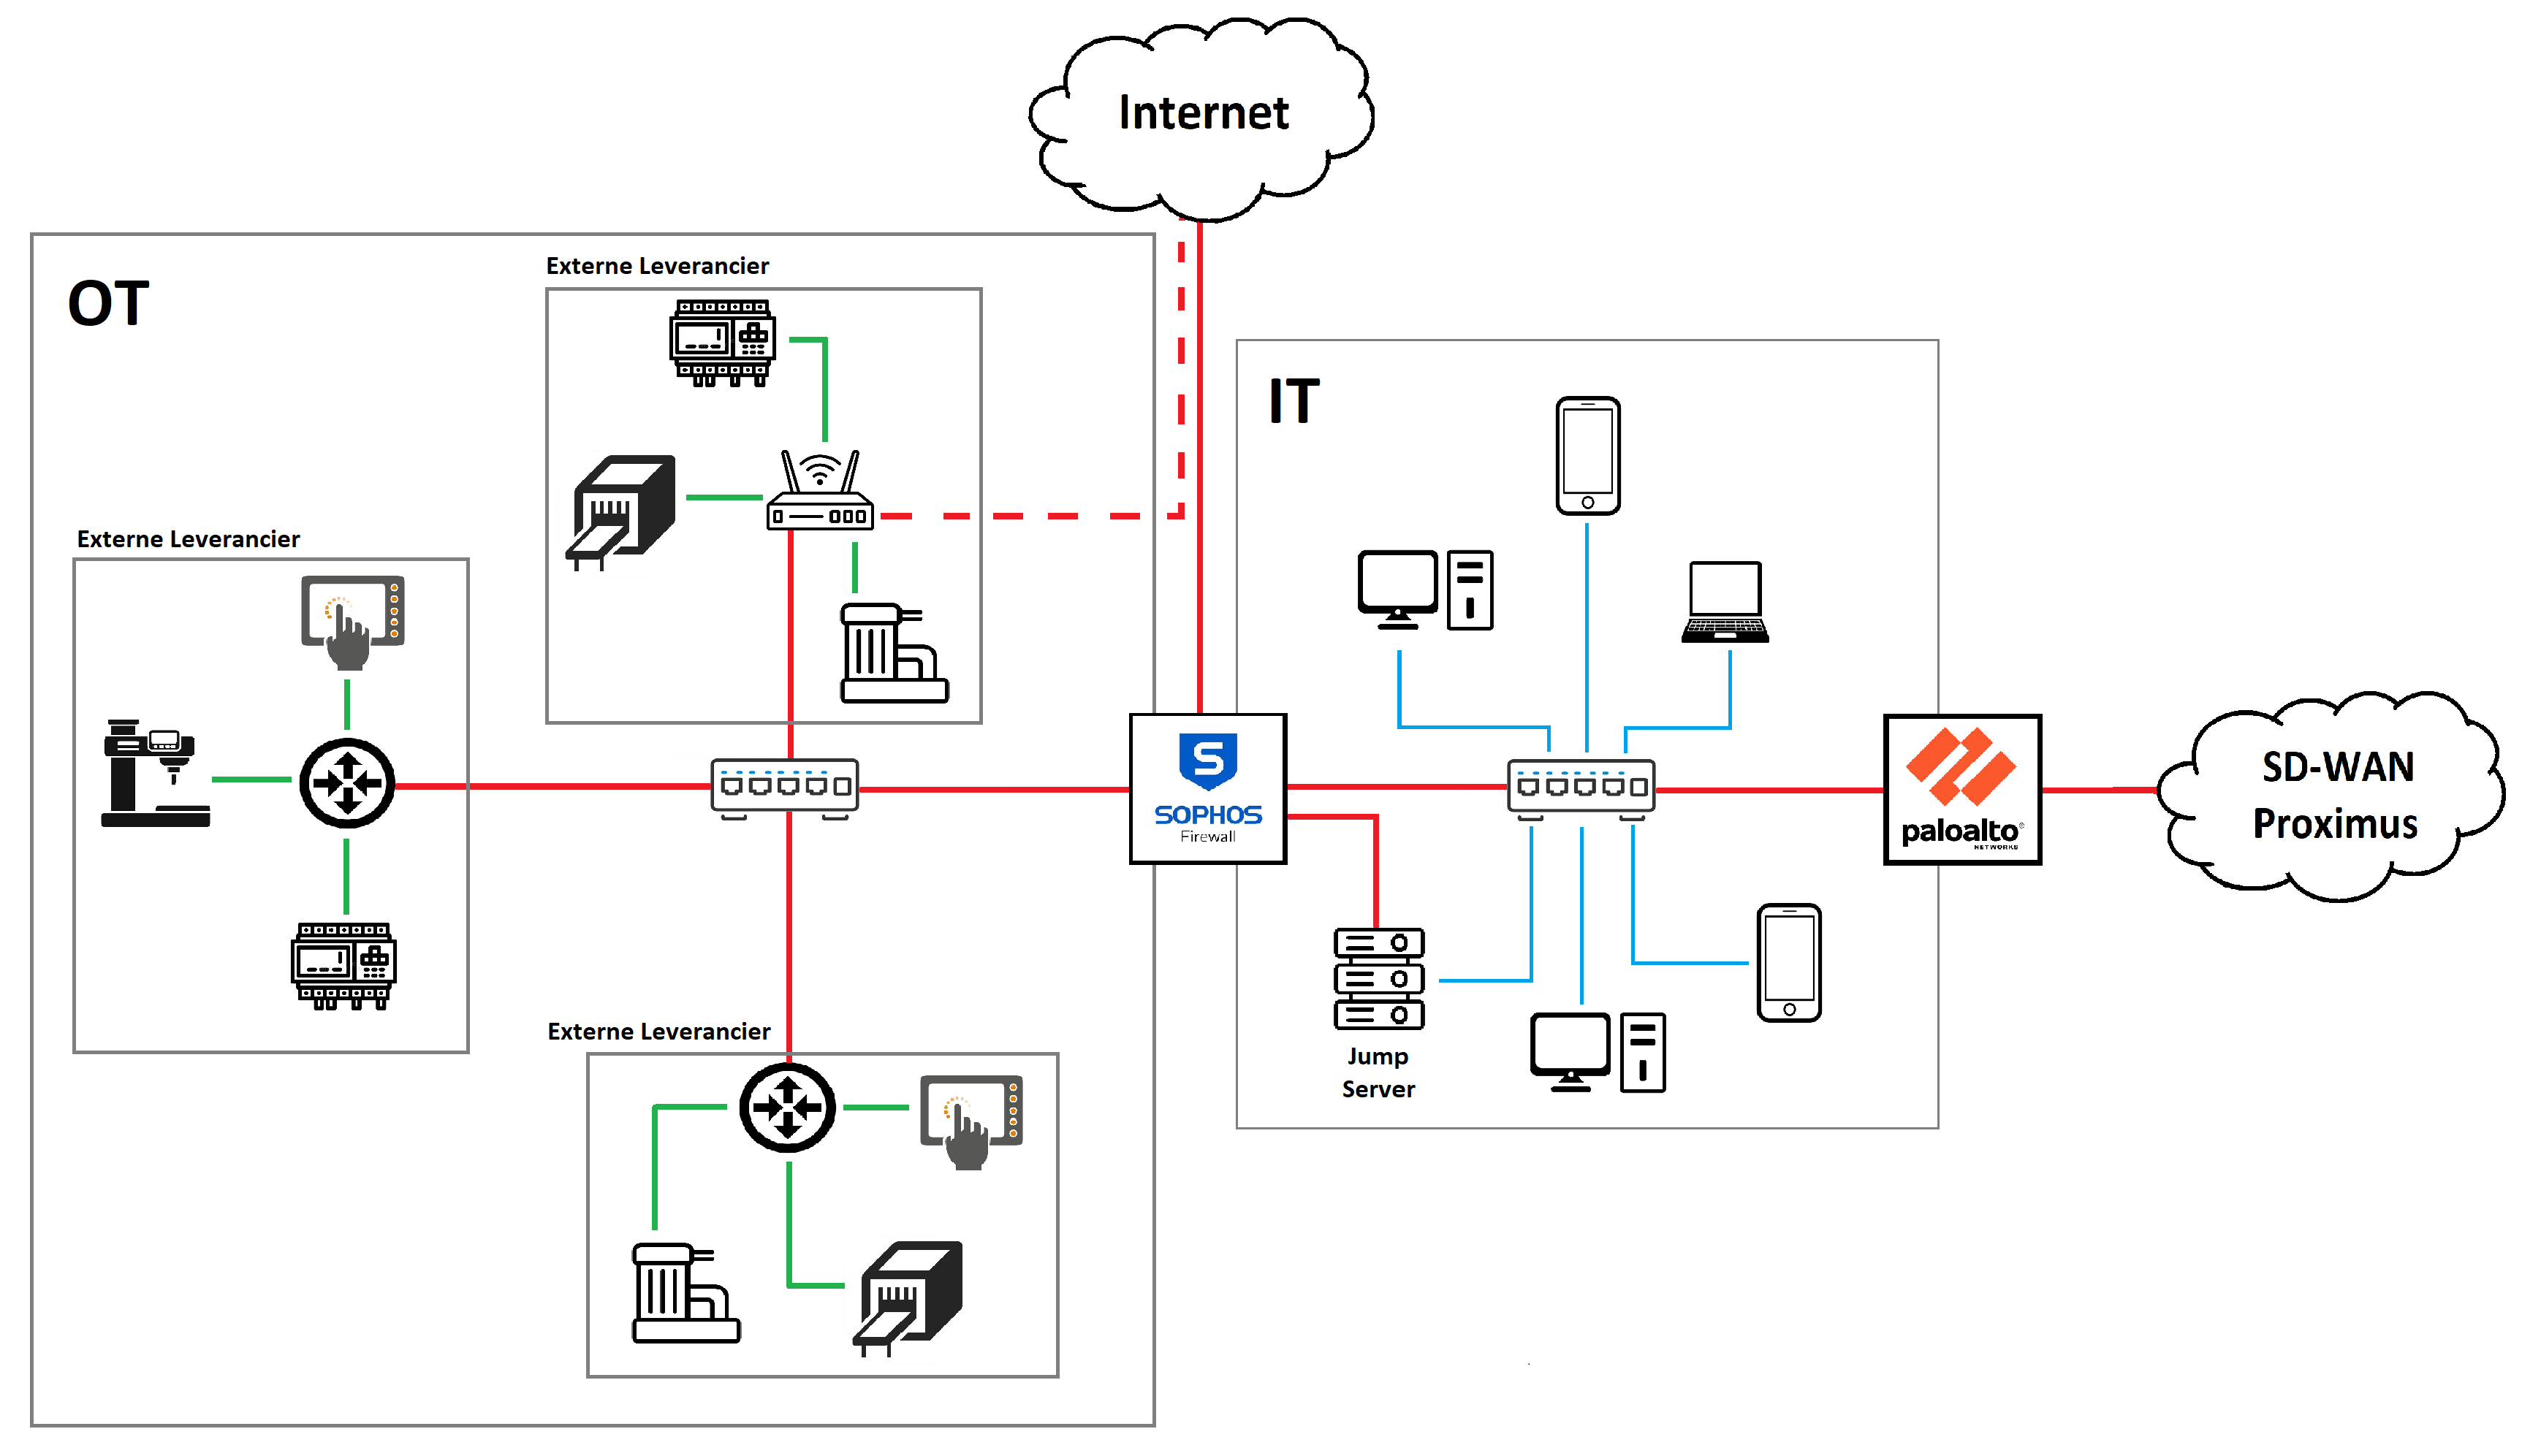
\includegraphics[width=0.8\textwidth]{fotos/FR16_before.png}%
    }
    \caption[high-level overzicht]{\label{fig:grail}Een high-level overzicht van het netwerk werd opgesteld om snel en duidelijk inzicht te geven in de huidige staat van de infrastructuur.}
\end{figure}


\subsection{Problemen met huidige OT Firewall opstelling}
Om te beginnen is het OT-netwerk van deze site beveiligd met een firewall van het merk Sophos. Dit vormt een uitdaging, aangezien VPK standaard gebruikmaakt van Palo Alto firewalls voor de beveiliging van alle andere productiesites die ze beheren. Palo Alto biedt een centrale webinterface, genaamd Strata Cloud Manager(SCM), waarmee alle geïmplementeerde firewalls binnen het netwerk op één platform kunnen worden beheerd.

Omdat Sophos firewalls niet compatibel zijn met SCM, moeten ze afzonderlijk worden beheerd via een eigen online portaal. Dit leidt tot een versnipperde beheersomgeving, waarin netwerkbeheerders meerdere systemen moeten gebruiken om de verschillende firewalls te beheren. Hierdoor neemt de complexiteit toe en wordt het lastiger om een uniforme beveiligingsstrategie te hanteren.

Een bijkomend voordeel van Strata Cloud Manager is dat het niet alleen een centraal overzicht biedt van alle Palo Alto firewalls, maar ook de mogelijkheid geeft om firewallregels op één plek te beheren en automatisch uit te rollen naar specifieke firewalls binnen het netwerk. Dit maakt het eenvoudiger om wijzigingen consistent door te voeren en minimaliseert de kans op fouten bij handmatige configuraties.
Daarnaast kan het gebruik van verschillende firewallmerken leiden tot inconsistente security policies, verhoogde operationele lasten en een grotere kans op menselijke fouten bij configuraties en monitoring. Om een efficiënter en gestroomlijnder netwerkbeheer te realiseren, zou het migreren van de Sophos firewall naar een andere firewalloplossing, zoals Palo Alto, een logische volgende stap zijn.

Daarnaast heeft niemand binnen het huidige netwerkteam van VPK ervaring met het implementeren en configureren van Sophos firewalls. Hoewel dit op dit moment geen direct probleem vormt voor de huidige firewallopstelling, is het wel een belangrijke factor om in overweging te nemen. Op langere termijn kan het gebrek aan expertise leiden tot verschillende uitdagingen, zoals een incorrecte configuratie van de firewalls door onvoldoende kennis van de specifieke implementatie- en beheersprincipes van Sophos.

Een verkeerde configuratie kan resulteren in beveiligingsrisico’s, verminderde netwerkprestaties of zelfs netwerkstoringen. Om deze risico’s te beperken, kan er overwogen worden om over te stappen op een firewalloplossing die beter aansluit bij de bestaande kennis en beheertools binnen VPK zoals een firewall van Palo Alto.\newline

\begin{figure}[H]
    \centering
    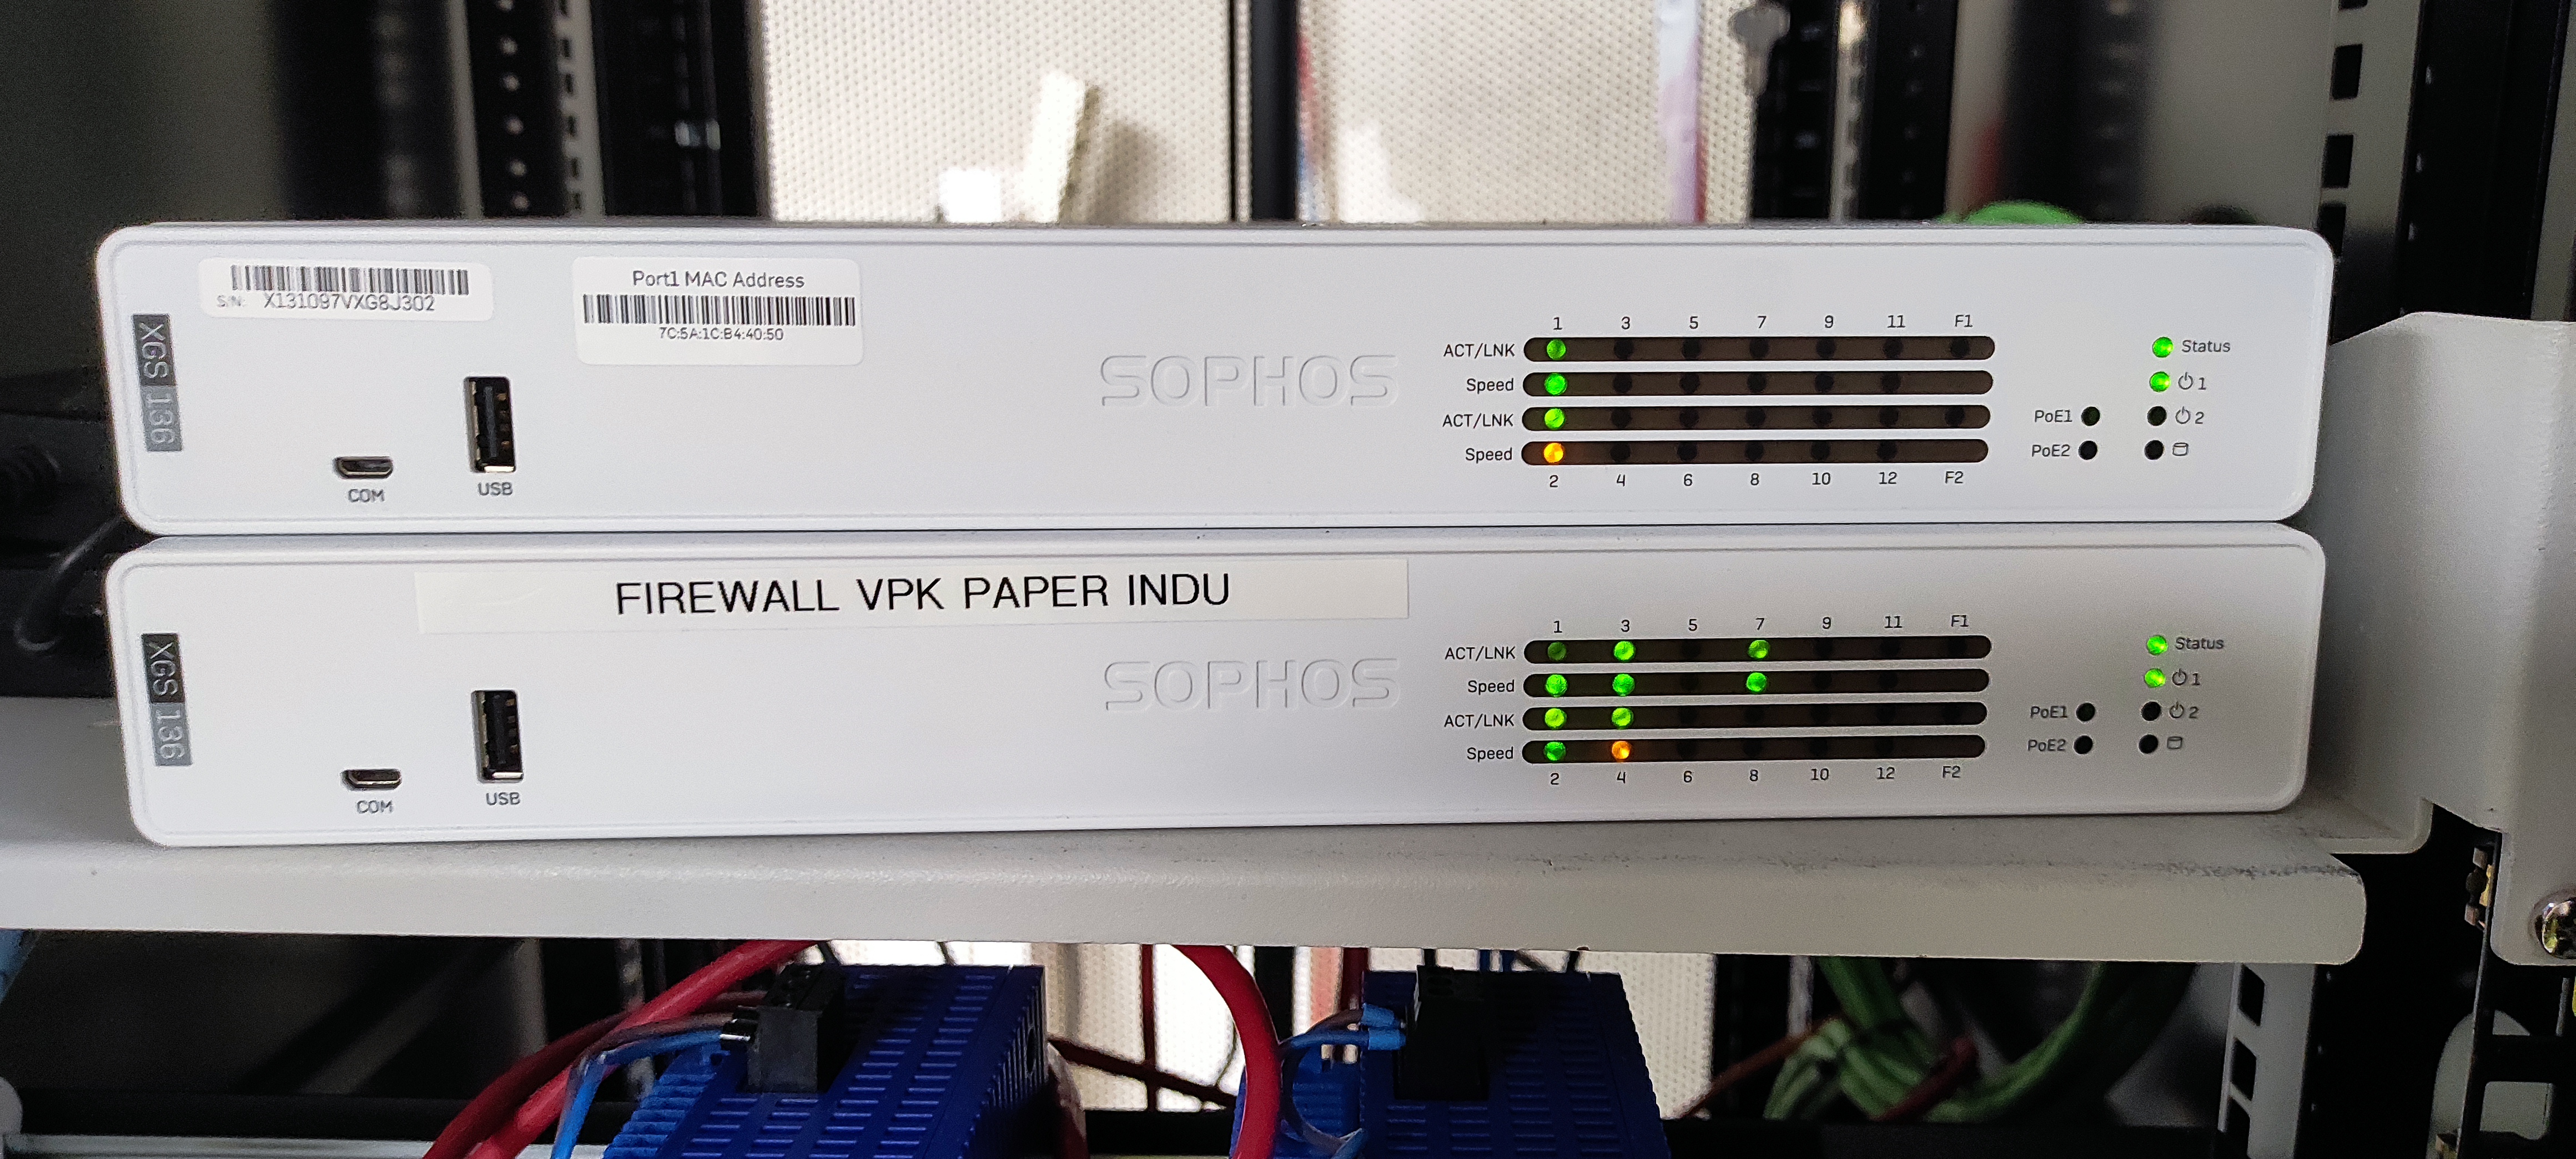
\includegraphics[width=0.8\textwidth]{fotos/SophosFirewall.jpg}
    \caption[Sophos Firewall]{\label{fig:grail}De huidige Sophos firewall die gebruikt wordt op de FR16 site van VPK.}
\end{figure} 

\subsection{Problemen met het huidige OT netwerk}
Een van de grootste uitdagingen binnen het netwerk van de productiesite van Alizay is het gebrek aan documentatie over de bestaande infrastructuur. Het netwerkteam dat verantwoordelijk was voor het onderhoud van het IT- en OT-netwerk voor de overname door VPK heeft geen gedetailleerde documentatie bijgehouden over de netwerkarchitectuur. Dit maakt het beheer van het netwerk moeilijker, omdat er onvoldoende inforimatie beschikbaar is over de werking en samenstelling ervan. Zonder deze kennis wordt het uitdagend om aanpassingen door te voeren, storingen snel op te lossen en beveiligingsrisico’s effectief te beheersen.
Het OT-netwerk binnen de site van Alizay bestaat uit meerdere generaties componenten die in de loop van tientallen jaren zijn geïmplementeerd. Hierdoor is het netwerk geleidelijk uitgebreid met verschillende subnetwerken die doorheen de jaren zijn toegevoegd, vaak zonder een plan of duidelijke standaardisatie. Dit heeft geleid tot een complexe en gefragmenteerde infrastructuur, waarbij verschillende systemen en protocollen naast elkaar bestaan.
Deze gelaagde netwerkstructuur kan verschillende uitdagingen veroorzaken wanneer wordt besloten de huidige firewallregels te herzien of te optimaliseren. Op dit moment zijn er geen specifieke firewallregels die expliciet bepalen welke data uit de verschillende subnetwerken mag worden doorgelaten of geblokkeerd. Dit betekent dat het netwerk mogelijk meer verkeer toestaat dan strikt noodzakelijk is, wat een potentieel beveiligingsrisico vormt. Tegelijkertijd zorgt het ontbreken van een duidelijke segmentatie van het netwerk ervoor dat ongewenste blokkades kunnen optreden wanneer nieuwe firewallregels worden ingevoerd.
De combinatie van een verouderde netwerkinfrastructuur en het gebrek aan een goed gedefinieerd firewallbeleid kan het risico met zich mee brengen dat bepaalde subnetwerken of systemen onverwacht worden geblokkeerd bij herconfiguratie van de firewall. Dit kan ertoe leiden dat machines tijdelijk uitvallen, wat een negatieve impact heeft op de productieprocessen en de volledige supply chain. In sommige gevallen kan zelfs een kleine onderbreking in de netwerkcommunicatie ervoor zorgen dat een machine niet meer correct functioneert, waardoor productiestilstand ontstaat en de continuiteit van de productie niet gewaarborgd kan worden.

Binnen de verschillende productiesites van VPK wordt gebruikgemaakt van machines afkomstig van diverse externe leveranciers. Deze geavanceerde machines bevatten vaak een combinatie van verschillende technische componenten, zoals PLC’s, sensoren, pneumatische systemen, robotarmen en geautomatiseerde transportsystemen zoals die van Minda. 

\begin{figure}[H]
    \centering
    \includegraphics[width=0.8\textwidth]{fotos/MindaConveyorFotoBP.jpg}
    \caption[Minda Conveyor]{\label{fig:grail} Een Minda conveyor installatie die pallets met kartonnen dozen verplaatst. ©Talina Scholz}
\end{figure} 

Deze componenten zijn onderling afhankelijk en wisselen continu data uit om productieprocessen op elkaar af te stemmen. Om deze gegevensuitwisseling mogelijk te maken moet er een betrouwbaar netwerk aanwezig zijn die alle verschillende componenten met elkaar verbindt.
In de praktijk betekent dit dat fabrikanten van deze machines vaak genoodzaakt zijn om hun eigen kleine netwerken op te zetten binnen de productiesite. Dit gebeurt met behulp van netwerkcomponenten zoals switches en routers, zodat hun machines correct kunnen functioneren. Wanneer een productiesite veel verschillende machines van uiteenlopende fabrikanten bevat, ontstaat al snel een situatie waarbij een groot aantal afzonderlijke private netwerken naast elkaar bestaat. Omdat deze netwerken zelden op elkaar worden afgestemd of gestandaardiseerd, leidt dit tot een uiterst gefragmenteerde netwerkstructuur. Hierdoor wordt het uniform beheren van de netwerken op verschillende VPK-sites vrijwel onmogelijk, aangezien elke site een unieke combinatie van leveranciers, machines en netwerktopologieën bevat.
Daarnaast vereisen veel fabrikanten een externe verbinding met hun machines om op afstand onderhoud te kunnen uitvoeren, real-time monitoring mogelijk te maken of software-updates te installeren. Dit betekent dat er op de productiesite van Alizay op twee mogelijke manieren een connectie met het internet kan worden gerealiseerd. De eerste optie is dat de fabrikant gebruikmaakt van het bestaande bekabelde netwerk van de site, dat wordt beheerd door VPK. In dit geval moet er bij de configuratie van de firewallregels rekening mee worden gehouden dat dit verkeer niet per ongeluk wordt geblokkeerd, anders verliest de fabrikant de mogelijkheid om zijn machines op afstand te beheren.
De tweede optie is dat de fabrikant een 4G-router met een eigen SIM-kaart gebruikt, zodat er geen directe verbinding met het netwerk van VPK nodig is. Hoewel dit in sommige gevallen een veiliger alternatief lijkt, introduceert het ook uitdagingen op het gebied van toezicht en controle over externe verbindingen. Soms kan het ook zijn dat een externe fabrikant gebruik maakt van een 4G-router en een fysieke verbinding met het VPK netwerk. In feite zal de fabrikant hierdoor de firewall gaan omzeilen. Dit is een uiterst kwetsbaar fenomeen dat veel schade kan berokken aan het VPK netwerk. Omdat in feite de firewall omzeild zal worden.
Beide methoden brengen aanzienlijke beveiligingsrisico’s met zich mee. Veel van de private netwerken die door machinefabrikanten worden opgezet, voldoen niet aan de meest recente cybersecuritystandaarden. Dit betekent dat ze kwetsbaar kunnen zijn voor aanvallen van buitenaf. Indien een hacker erin slaagt toegang te krijgen tot zo’n slecht beveiligd netwerk, kan dit een potentiële ingang vormen naar het bredere IT- en OT-netwerk van de productiesite. Dit zou ernstige gevolgen kunnen hebben, zoals productieonderbrekingen, verlies van kritieke data en zelfs de manipulatie van industriële processen.
\vspace{5mm} 

Naast de analyses die op afstand zijn uitgevoerd, heeft er ook een fysiek bezoek aan FR16 plaatsgevonden. Dit bezoek was noodzakelijk omdat het niet mogelijk was om het volledige fysieke netwerk van FR16 volledig in kaart te brengen via remote methoden. Tijdens het op afstand in kaart brengen van het netwerk stuitte men op enkele uitdagingen. Een van deze uitdagingen was het gebruik van unmanaged switches binnen het OT netwerk. Deze switches maken het ontdekken en beheren van een netwerk zeer moeilijk, omdat deze switches niet beheerbaar zijn en geen inzicht geven in welke apparaten op de poorten zijn aangesloten. Op een poort van een unmanaged switch zijn enkel MAC-adressen zichtbaar van de aangesloten apparaten, zonder verdere context of identificatie van de aangesloten apparaten. Bovendien is het niet mogelijk om in te loggen op de switch voor configuratie of monitoring, wat het traceren, beheren en analyseren van netwerkverbindingen aanzienlijk lastiger maakt.


\begin{figure}[H]
    \centering
    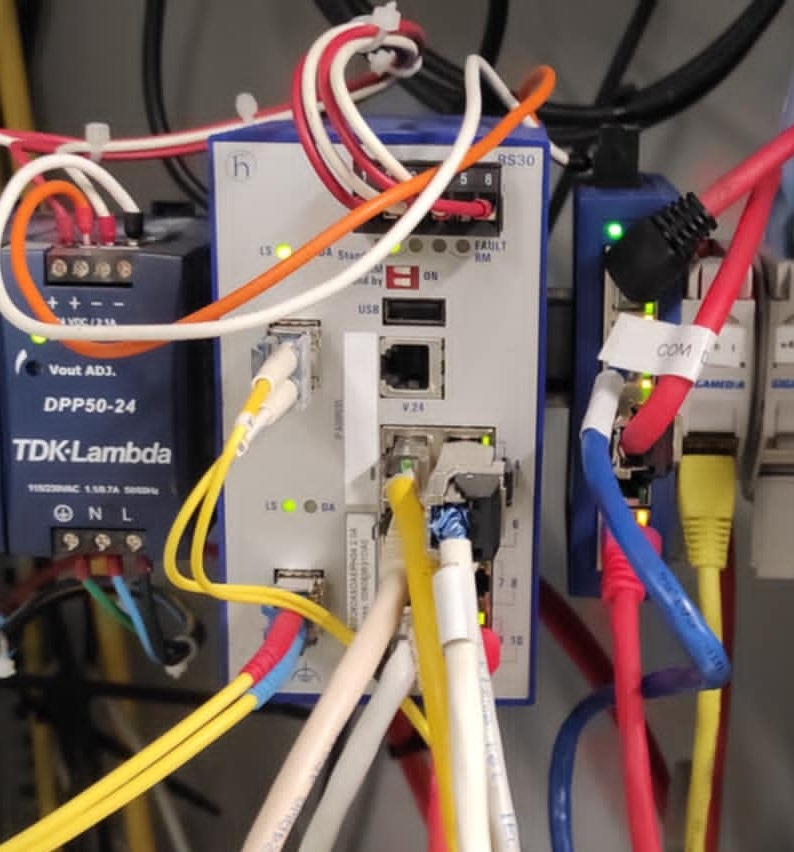
\includegraphics[width=0.8\textwidth]{fotos/hirschmannSwitch.jpg}
    \caption[Hirschmann switch]{\label{fig:grail} Een unmanaged Hirschmann switch die wordt gebruikt binnen het OT netwerk van de FR16 site van VPK.}
\end{figure}


\section{Analyse van de gewenste opstelling}
Binnen de huidige opstelling functioneren het OT en IT netwerk als twee afzonderlijke systemen die los van elkaar opereren. Deze scheiding is echter niet de meest efficiënte oplossing. Een betere benadering zou zijn om beide netwerken binnen één geïntegreerde infrastructuur onder te brengen, beheerd via een centrale firewall. Hierdoor kunnen het OT en IT netwerk effectief van elkaar worden gescheiden door gebruik te maken van verschillende VLAN’s. Dit is een mmethode die bekend staat als netwerksegmentatie. In onderdeel ONDERDEELNUMMER wordt hier dieper op ingegaan.

\begin{figure}[H]
    \centering
    \fbox{%
        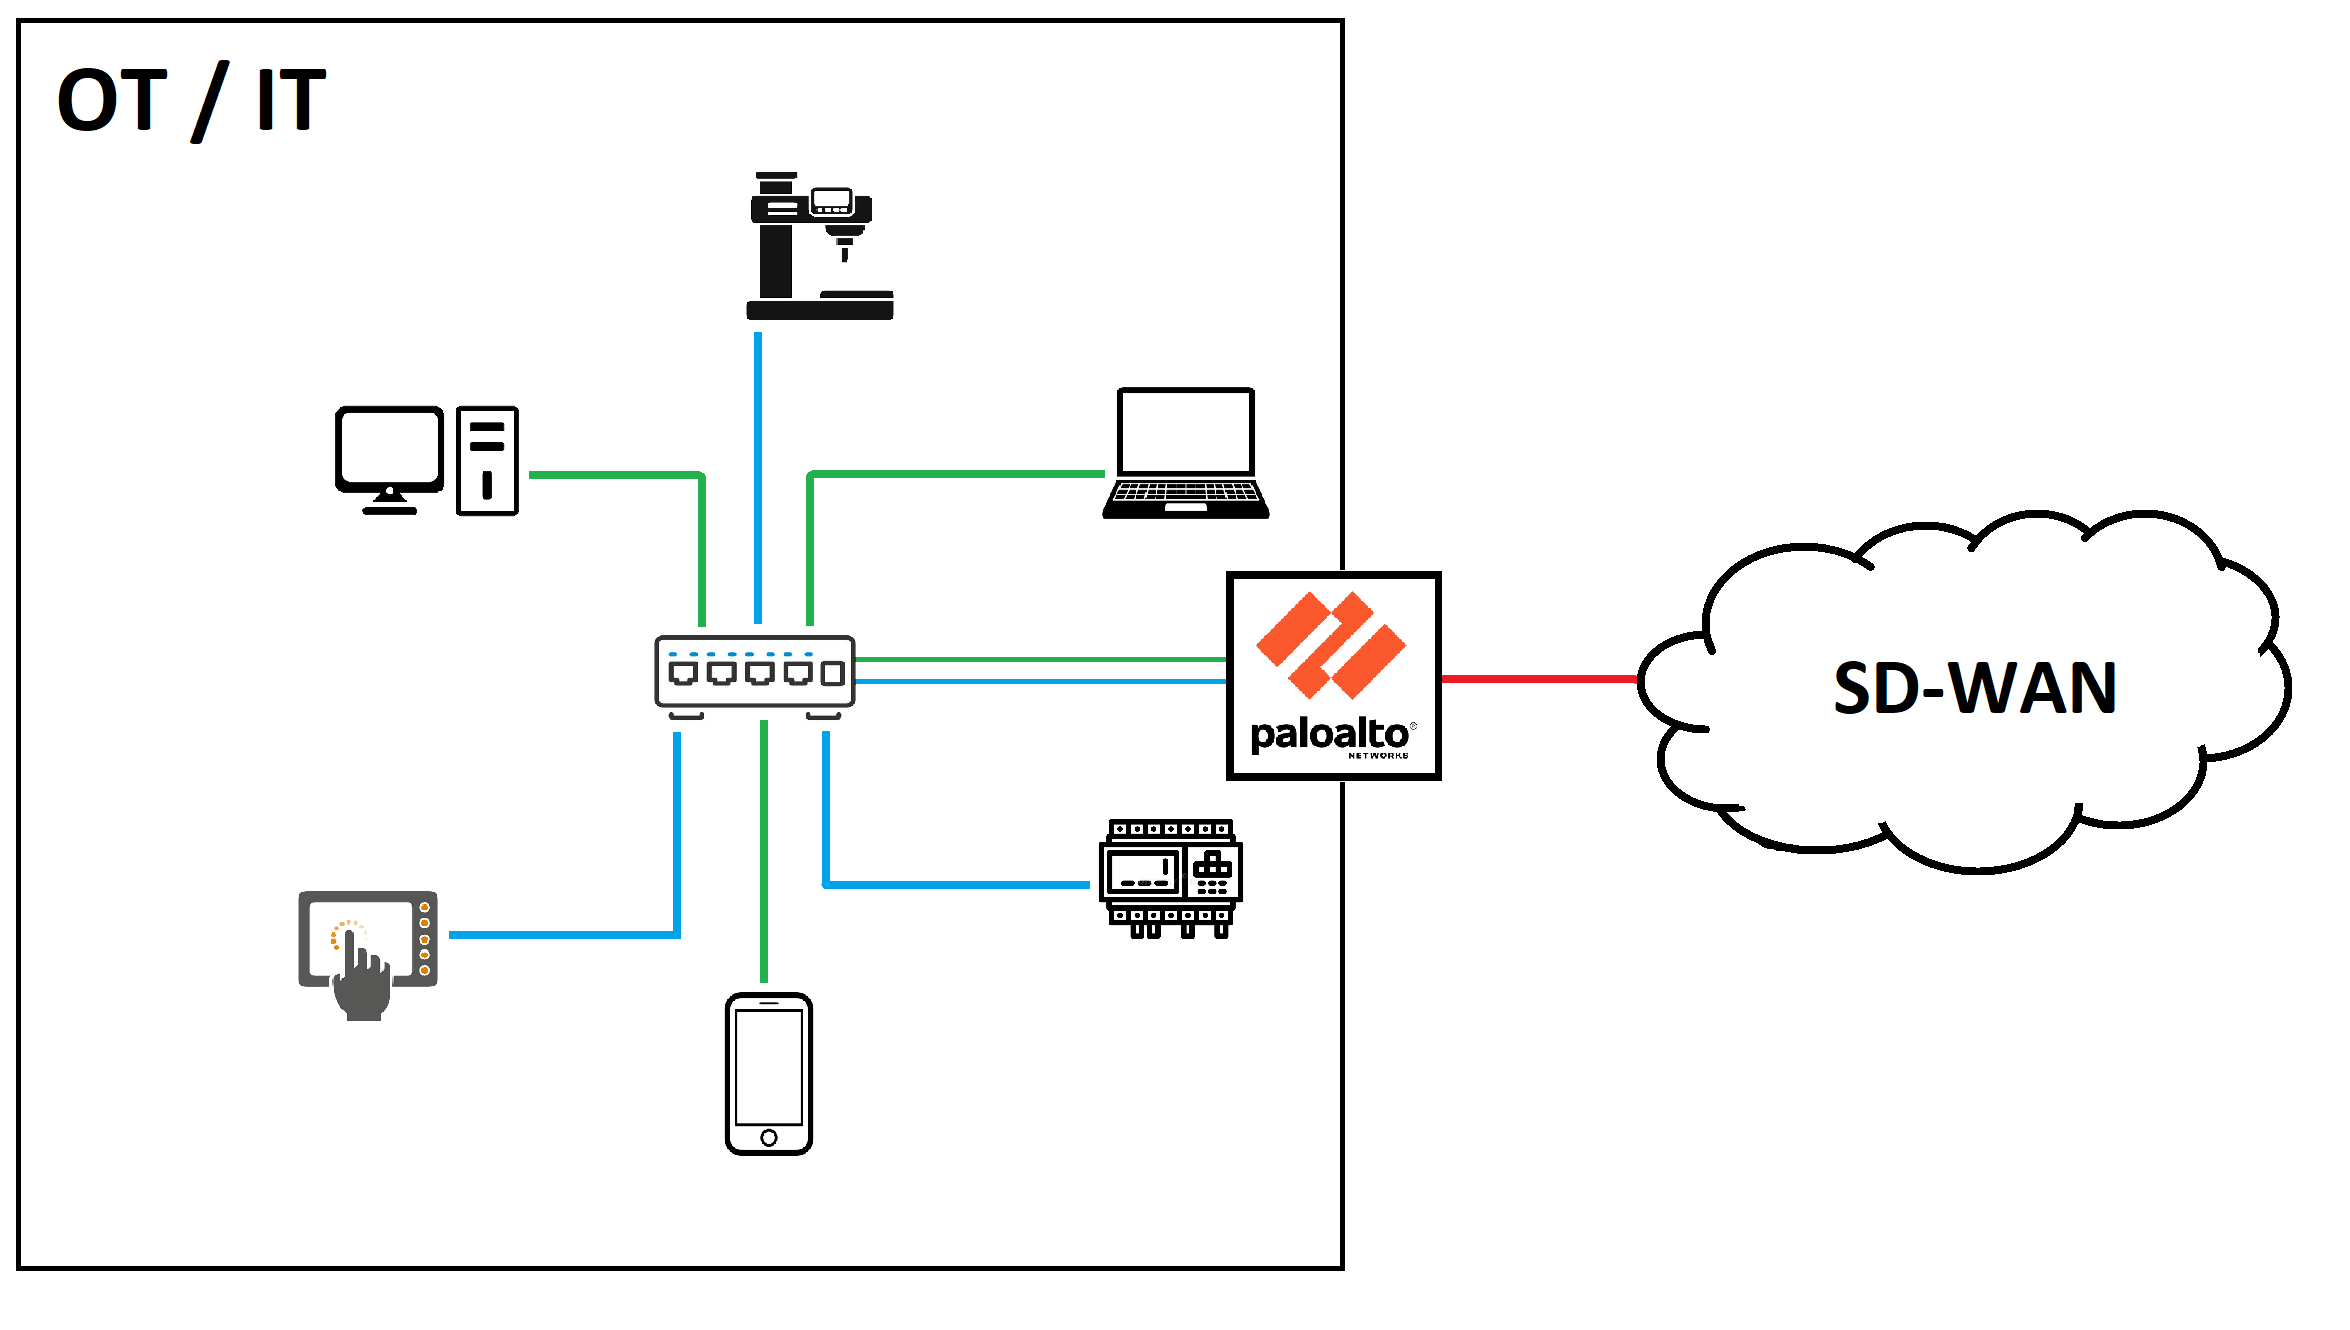
\includegraphics[width=0.8\textwidth]{fotos/FR16_after.png}%
    }
    \caption[high-level overzicht]{\label{fig:grail}Een high-level overzicht van hoe het gewenste OT/IT netwerk er zou uitzien mocht er gekozen worden om een Palo Alto firewall te implementeren.}
\end{figure}


\section{SWOT Analyse van de huidige situatie}
In dit deel zal er een SWOT analyse worden opgesteld op basis van de huidige situatie van het netwerk.


\subsection{Strengths}
\begin{itemize}
\item \textbf{Extra laag bescherming:} Er is al een Palo Alto (PA) firewall aanwezig, wat betekent dat de Sophos firewall een extra laag van bescherming biedt. Dit is positief omdat het netwerk al enige beveiliging heeft, en de extra firewall kan helpen om de beveiliging verder te versterken.

\item \textbf{De setup werkt, ook al is hij niet optimaal:} De huidige netwerkconfiguratie werkt wel, ook al is hij niet perfect. Dit betekent dat er geen grote storingen of onderbrekingen zijn, maar er is nog ruimte voor verbetering.


\end{itemize}

\subsection{Weaknesses}

\begin{itemize}
\item \textbf{Complexiteit door de Sophos firewall:} De Sophos firewall maakt het netwerkbeheer onnodig complex. Deze firewall voegt weinig extra waarde toe, maar maakt troubleshooting en het algemene beheer moeilijker. Binnen het huidige IT team van VPK is er niemand aanwezig die uitgebreide kennis heeft over de werking van een Sophos firewall.

\item \textbf{Gebrek aan documentatie:} Het netwerk is slecht gedocumenteerd en niemand binnen het OT/IT team van Alizay kent de volledige netwerktopologie. Dit maakt het lastig om het netwerk te beheren, te troubleshooten of wijzigingen door te voeren zonder risico’s.

\item \textbf{Slechte firewallconfiguratie:} De huidige configuratie van de Sophos firewall is niet optimaal. Er zijn onnodige statische routes en ineffectieve firewallregels, wat zorgt voor extra complexiteit en mogelijk ook kwetsbaarheden in de beveiliging.

\item \textbf{Verouderde switches:} De HP switches die al sinds 2002 in gebruik zijn, hebben geen updates meer ontvangen. Dit maakt ze kwetsbaar voor beveiligingsrisico’s en zorgt ervoor dat ze niet optimaal functioneren. Ook zal hun ouderdom er voor zorgen dat er een grotere kans is op het falen van één of meerdere van hun onderdelen. Hierdoor is de kans dat er een outage is van één van deze devices een pak groter. 
\end{itemize}
    
\subsection{Opportunities}




\subsection{Threats}

\begin{itemize}
\item \textbf{De Sophos firewall is een zwakke schakel in het netwerk:} Doordat de Sophos-firewall niet correct is beheerd, zijn er verschillende kwetsbaarheden ontstaan die een aanvaller zou kunnen misbruiken. Denk hierbij aan verouderde firmware, slecht geconfigureerde firewallregels en zwakke beheerderswachtwoorden.

\item \textbf{netwerk is niet up-to-date met NIS2 richtlijnen} Het OT-netwerk van FR16 is niet in overeenstemming met de actuele NIS2-richtlijnen. Zo wordt onder andere niet voldaan aan PR.IP-3, een onderdeel dat vereist dat alle netwerkwijzigingen in overeenstemming zijn met een formeel wijzigingsbeheerbeleid. In de praktijk ontbreekt er documentatie over het netwerk, wat duidt op een gebrek aan structureel beheer en controle.

\item \textbf{Impact op dienstverlening van externe partners:} Er zijn veel externe partners die met het netwerk verbonden zijn, zoals S2I, Evrest, en Valmet. Zij hebben netwerktoegang nodig om op afstand onderhoud uit te voeren, updates te installeren of eerstelijnsproblemen op te lossen.
\end{itemize}


\section{SWOT Analyse van de gewenste opstelling}
In dit deel zal er een SWOT analyse worden opgesteld op basis van de gewenste situatie van het netwerk.


\subsection{Strengths}
\begin{itemize}
    \item \textbf{Toegang enkel mogelijk via een goed beveiligde Palo Alto firewall.} Aangezien het gewenste netwerk slechts één, goed beveiligde Palo Alto firewall bevat is de algemene netwerkbeveiliging versterkt. De zwakke schakel, de eerder gebruikte Sophos firewall, is daarmee verwijderd uit het netwerk waardoor het risico op ongeautoriseerde toegang aanzienlijk is verminderd.
    
    \item \textbf{Het netwerk is uniform aan andere VPK sites} De gewenste netwerkopstelling sluit aan bij de configuraties die ook op andere VPK sites worden gebruikt. Dit zorgt voor meer uniformiteit, waardoor wijzigingen efficiënter kunnen worden doorgevoerd en troubleshooting eenvoudiger en met minder kans op fouten verloopt.

    \item \textbf{De EoL netwerapparaten zijn vervangen.} De meeste netwerkapparaten in dit netwerk hebben hun EoL datum ruim overschreden. Deze zullen daarom worden vervangen door nieuwere, ondersteunde modellen om de betrouwbaarheid en veiligheid van het netwerk te waarborgen.
    
\end{itemize}

\subsection{Weaknesses}

\begin{itemize}
    \item \textbf{Samenwerking tussen meerdere stakeholders:} Omdat het OT en IT netwerk worden samengevoegd tot één groot netwerk zullen verschillende stakeholders zullen moeten samenwerken om het netwerk te beheren. 
    
    \item \textbf{Overlap van bepaalde taken binnen het OT/IT netwerk:} Door de samenvoeging van de twee netwerken ontstaat er overlap in bepaalde taken. Met behulp van een RASCI tabel worden de verantwoordelijkheden duidelijk vastgelegd, waardoor verwarring wordt voorkomen en de samenwerking soepel verloopt.
    
    \item \textbf{Knowledge gap tussen IT en OT:} OT en IT zijn twee verschillende domeinen, waardoor de betrokken stakeholders vaak over uiteenlopende kennis beschikken. Dit verschil kan de samenwerking tussen OT en IT teams bemoeilijken.
    
\end{itemize}

\subsection{Opportunities}

\begin{itemize}
    \item \textbf{Remote toegang voor externe leveranciers via de firewall} De toegang voor externe leveranciers kan optimaal worden ingericht via de firewall. Deze toegang wordt zorgvuldig beheerd. Hierdoor kunnen leveranciers eenvoudig op afstand toegang krijgen tot hun machines, zonder dat er nog gebruik hoeft te worden gemaakt van 4G routers.
    
    \item \textbf{NIS2 kan worden toegepast} Door het netwerk aan te passen, kunnen de verschillende NIS2-richtlijnen worden nageleefd. Zo zal bijvoorbeeld aan PR.IP-3 worden voldaan door het netwerk voortaan direct en volledig te documenteren.
    
\end{itemize}


\subsection{Threats}

\begin{itemize}
    \item \textbf{wip:} wip
    
\end{itemize}



\section{RASCI Analyse}

Volgens \textcite{Epam2024} is RASCI een raamwerk dat specifieke rollen en verantwoordelijkheden toekent aan belanghebbenden die betrokken zijn bij een project of proces. Zie het als een routekaart die iedereen naar een gezamenlijk doel leidt zonder verwarring of vertraging. 
De verschillende letters van RASCI staan voor een bepaald woord dat een bepaalde rol samenvat.

\begin{itemize}
    \item \textbf{Responsible:} De rol die de taak effectief uitvoert. Deze persoon of groep is de drijvende kracht achter de uitvoering van de taak. 
    \item \textbf{Accountable:} De eindverantwoordelijke voor de taak. Deze rol draagt de verantwoordelijkheid voor het uiteindelijke succes of falen van de taak. 
    \item \textbf{Supportive:} Een rol die ondersteuning biedt aan de 'Responsible' bij het uitvoeren van de taak. 
    \item \textbf{Consulted:} Een persoon of rol die waardevolle input levert. Zij worden geraadpleegd voor advies en meedenken bij belangrijke beslissingen.
    \item \textbf{Informed:} De rol die op de hoogte wordt gehouden van beslissingen of acties die binnen de taak plaatsvinden.
\end{itemize}

\subsection{Opbouw van de RASCI Matrix.}
Volgens \textcite{Cabanillas2011} is een RASCI-matrix is opgebouwd uit twee assen: op de horizontale as worden de verschillende rollen binnen het project weergegeven, terwijl de verticale as de diverse taken toont. In elk vakje van de matrix wordt met een enkele letter aangeduid welke rol welke verantwoordelijkheid opneemt voor een bepaalde taak. Zo staat bijvoorbeeld de letter 'R' voor "Responsible. Wanneer bijvoorbeeld de letter 'R' in een bepaald vakje voorkomt, betekent dit dat de overeenkomstige rol op de horizontale as Responsable is voor de taak op de verticale as. \autocite{Cabanillas2011}

\subsection{Verschillende taken binnen deze RASCI matrix}

\textbf{Onderhouden documentatie van het OT netwerk.}
\begin{itemize}[label=\textbullet]
    \item Wanneer er wijzigingen plaatsvinden binnen het netwerk (zoals het toevoegen of verwijderen van apparaten) wordt de inventarisatie hierop aangepast. Het doel is om steeds te beschikken over een actueel netwerkplan van het OT netwerk, zodat de documentatie up-to-date blijft. 
\end{itemize}

\textbf{1st line support bieden.}
\begin{itemize}[label=\textbullet]
    \item  First-line support betreft het bieden van eerste hulp bij technische problemen of meldingen. De verantwoordelijke persoon is het eerste aanspreekpunt en probeert de meldingen zo snel en efficiënt mogelijk op te lossen, of indien nodig door te verwijzen naar een volgende ondersteuningslijn.
\end{itemize}

\textbf{Beheren van netwerkkasten externe leverancier}
\begin{itemize}[label=\textbullet]
    \item Binnen de OT-omgeving bevinden zich meerdere netwerkkasten met apparatuur van externe leveranciers, waaronder switches, routers en VPN-routers. Deze componenten zijn essentieel voor de werking van de productie-installaties. 
\end{itemize}

\textbf{Beheren van fysieke componenten binnen het OT netwerk.}
\begin{itemize}[label=\textbullet]
    \item Deze taak richt zich op het beheer van industriële hardware binnen het OT-netwerk, zoals industriële switches, PLC’s, SCADA-systemen, sensoren, en andere verbonden componenten die een directe rol spelen in de operationele processen.
\end{itemize}


\textbf{Beheren van fysieke componenten binnen het IT netwerk.}
\begin{itemize}[label=\textbullet]
    \item De fysieke componenten waar men het hier over heeft zullen voornamelijk bestaan uit: switches, routers, firewalls, servers, bekabeling, …
\end{itemize}

\textbf{Onderhouden OT firewall.}
\begin{itemize}[label=\textbullet]
    \item Binnen de huidige OT opstelling van FR16 is er een Sophos firewall aanwezig. Deze firewall wordt enkel gebruik binnen het OT netwerk. Daarom is het OT team verantwoordelijk voor het beheer van deze firewall.
\end{itemize}



\begin{figure}[H]
    \centering
    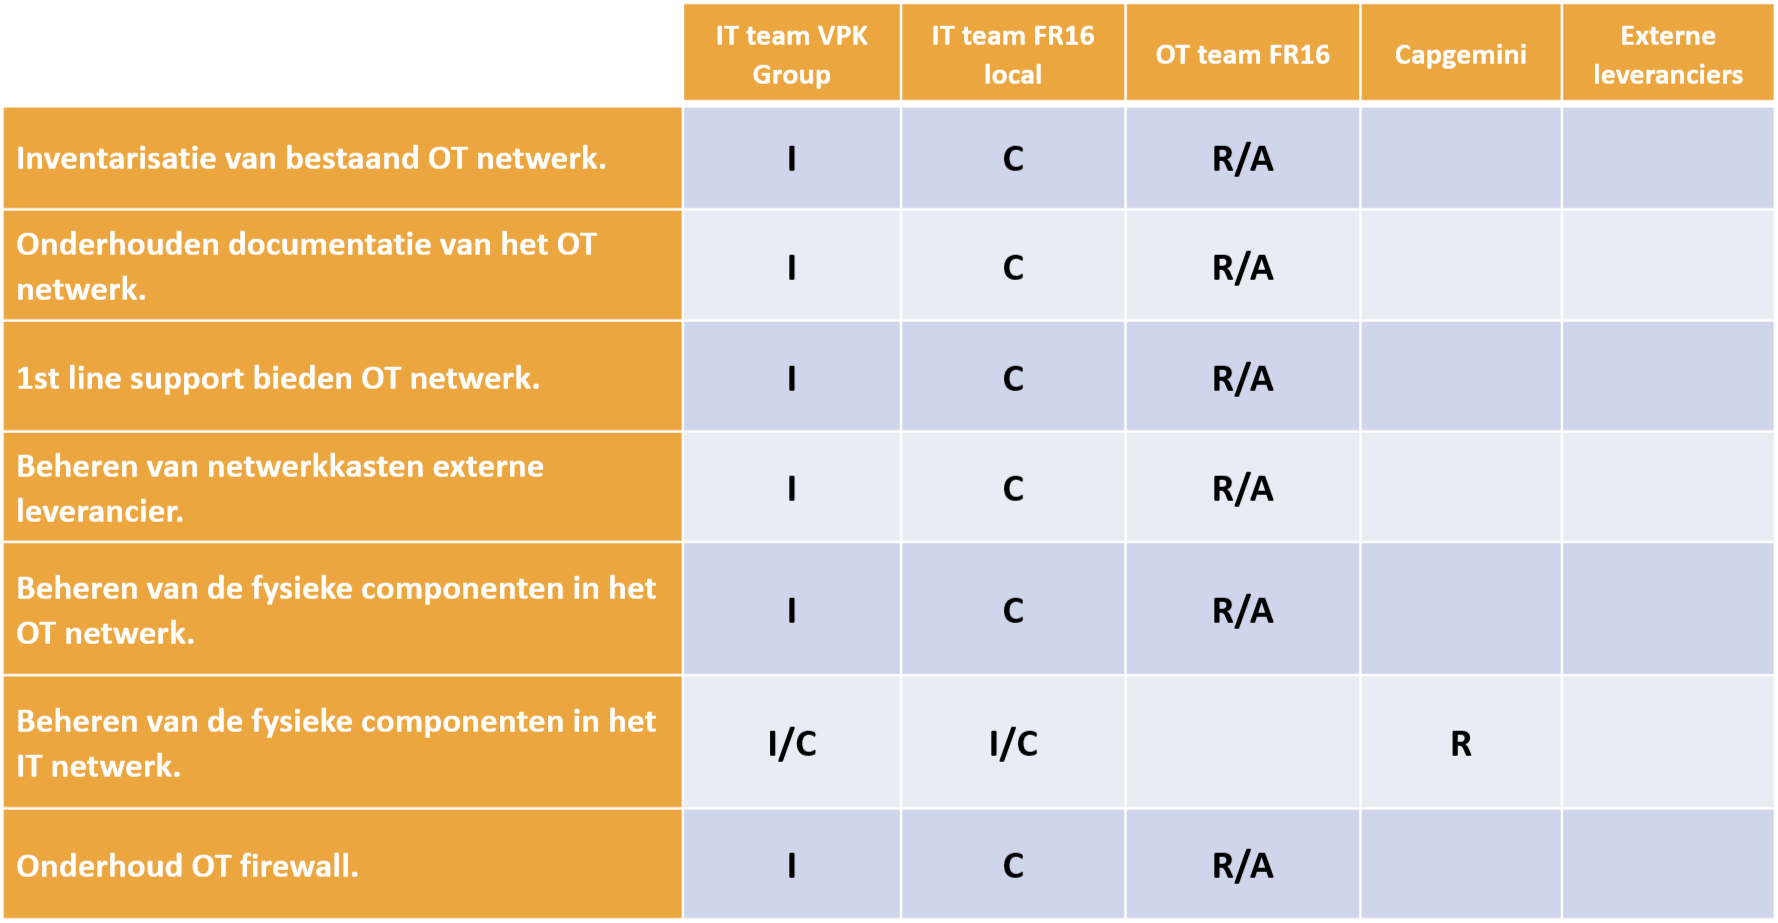
\includegraphics[width=1\textwidth]{fotos/Rasci_AS-IS.png}
    \caption[Foto Rasci AS-IS]{\label{fig:grail}Rasci tabel van de huidige toestand in FR16.}
\end{figure} 

\begin{figure}[H]
    \centering
    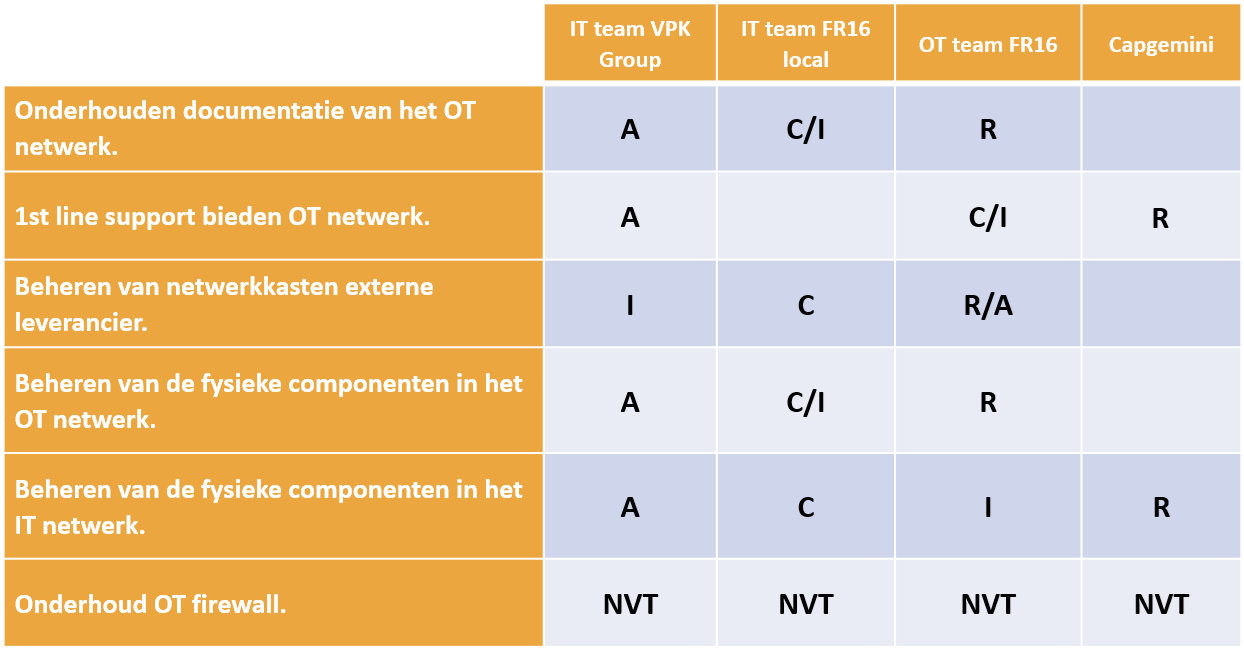
\includegraphics[width=1\textwidth]{fotos/Rasci_TO-BE.png}
    \caption[Foto Rasci TO-BE]{\label{fig:grail}Rasci tabel voor de toekomstige opstelling in FR16.}
\end{figure} 


\subsection{Doel van de nieuwe RASCI tabel}
In de huidige (AS-IS) RASCI-tabel is het OT-team van FR16 verantwoordelijk voor alle taken. Omdat dit team vaak onvoldoende kennis heeft van IT systemen, leidt dit regelmatig tot wanbeheer van IT apparatuur binnen de OT omgeving. \newline
Daarom is ervoor gekozen om de verantwoordelijkheden opnieuw te verdelen. Elke stakeholder binnen het netwerk zal voortaan taken uitvoeren die aansluiten bij zijn of haar expertise. Deze nieuwe verdeling zal leiden tot een efficiëntere werking van het OT en IT netwerk binnen FR16.

Daarnaast zal er ook een verschuiving zijn van de accountability richting het IT team van VPK Group. Dit brengt verschillende voordelen met zich mee:

\begin{itemize}
    \item \textbf{Meer controle over wijzigingen:} Alle veranderingen aan het netwerk worden centraal gecoördineerd en goedgekeurd, waardoor ongeplande of ongeautoriseerde aanpassingen worden voorkomen.

    \item \textbf{Verbeterde standaardisatie:} Door de centrale aansturing sluit het beheer van het netwerk beter aan op de standaarden en best practices die binnen de hele VPK Group gelden.
    
    \item \textbf{Betere risicobeheersing: }Het IT team van VPK Group beschikt over meer ervaring op het gebied van cybersecurity en compliance dan het OT team van FR16. Zij zullen verantwoordelijk zijn voor de implementatie van richtlijnen zoals NIS2, wat bijdraagt aan een beter beveiligd en beter beheerd netwerk.
\end{itemize}

\chapter{Vergelijken van de PA en Sophos firewall}


\section{RFP als leidraad voor doordachte keuzes.}
Sinds 2015 maakte VPK gebruik van stateful firewalls zonder NGFW functionaliteiten. Om de overstap te maken naar next generation firewalls (NGFW), diende VPK een Request for Proposal (RFP) in bij zowel Telenet als Proximus. In deze RFP werden diverse criteria opgenomen waaraan een toekomstige NGFW moest voldoen om in aanmerking te komen voor implementatie op alle VPK sites.

De destijds opgestelde RFP blijft vandaag de dag nog steeds relevant en kan nog steeds dienen als basis voor een doordachte keuze bij het maken van een eventuele overstap naar een andere NGFW. In deze studie zullen daarom verschillende criteria uit die oorspronkelijke RFP worden gebruikt om de functionaliteiten van de huidige Sophos en Palo Alto firewalls met elkaar te vergelijken.




\section{Vergelijking van verschillende firewall functionaliteiten}
In dit onderzoek maken we gebruik van twee verschillende firewalls om een vergelijking te kunnen maken. Voor Palo Alto gebruiken we de PA-440, aangezien dit type firewall het meest is geïmplementeerd op de meeste VPK productiesites. Voor Sophos gebruiken we de XGS 136, omdat deze firewall momenteel actief is binnen het OT-netwerk van de FR16-site.

In de RFP die VPK in 2015 heeft opgesteld, worden meer dan 150 criteria voorgesteld. Deze studie is echter niet uitgebreid genoeg om alle criteria waaraan NGFW’s moeten voldoen grondig te vergelijken. Daarom hebben verschillende IT professionals binnen VPK een lijst opgesteld met de belangrijkste criteria waaraan een moderne firewall moet voldoen. Beide firewalls zullen worden vergeleken aan de hand van de lijst met vooropgestelde criteria.




\subsection{Product provides Next-Generation Firewall functionality}

Binnen deze criteria zullen de twee firewalls worden vergeleken op basis van hun mogelijkheden binnen het gebruiken van NGFW functies. Waar we vooral op gefocust zullen zijn is het vergelijken van de verschillende cloud gebaseerde threat intelligence oplossingen die beide vendoren aanbieden.


\textbf{Palo Alto}
\begin{itemize}[label=\textbullet]
    \item Palo Alto maakt gebruik van AutoFocus, een threat intelligence-platform dat geavanceerde contextuele dreigingsinformatie biedt op basis van wereldwijde data, inclusief informatie van Unit 42. Unit 42 is het threat research team van Palo Alto. AutoFocus zorgt ervoor dat beveiligingsteams in staat zijn om snel te reageren op bedreigingen door automatisch verbanden te leggen tussen nieuwe aanvallen, Indicators of Compromise (IOC) en bekende dreigingsactoren. Dit gebeurt aan de hand van zeer specifieke kenmerken van aanvallen, in combinatie met ML.\autocite{PaloAltoAF2025}
    
    Om Autofocus te gebruiken moet men een extra licentie aankopen, de standaard Autofocus licentie die één jaar geldig is kost 31.000 euro per jaar, deze licentie is echter wel geldig voor alle PA firewalls binnen het netwerk. De prijs die je per firewall zal moeten betalen voor deze licentie hangt dus grotendeels af van het aantal actieve firewalls.
\end{itemize}

\textbf{Sophos}
\begin{itemize}[label=\textbullet]
    \item Sophos gebruikt Intelix, een cloudgebaseerde threat analysis service die ML en sanboxing combineert om zowel bekende als onbekende bedreigingen te detecteren. De focus van Intelix ligt vooral op het analyseren van individuele bestanden en e-mailbijlagen in een gecontroleerde omgeving. Hieruit genereert Intelix automatisch gedetailleerde risicorapporten die worden gebruikt voor zero-day bescherming. Deze technologie wordt vooral toegepast bij het uploaden van verdachte bestanden of inkomende e-mails, wat het een directe en hands-on analyseoplossing maakt. \autocite{SophosIN2025}
    
    Om gebruik te maken van Intelix, moet je beschikken over de Zero Day Protection bundel, die als aanvulling op de XDR-licentie wordt geleverd. De kosten hiervan zijn afhankelijk van de licentievorm en het aantal endpoints.
\end{itemize}



\subsection{Product provides traffic classification (Type of web traffic, etc)}

Binnen deze criteria worden de twee firewalls vergeleken op hun mogelijkheden tot traffic classification en traffic filtering. Hierbij analyseert de firewall het binnenkomende en uitgaande netwerkverkeer en deelt dit in op basis van verschillende kenmerken zoals: gebruikte poorten, protocollen, applicaties en bestemmingen. Op basis van deze indeling kan het verkeer vervolgens worden gefilterd. Zo kan de firewall specifieke websites of applicaties blokkeren, bijvoorbeeld sociale media, streamingsdiensten, goksites enzovoort afhankelijk van het beleid dat wordt ingesteld op de firewall.

Ook is het mogelijk om met deze indeling Quality of Service (QoS) in te stellen, zodat belangrijk verkeer zoals videobellen of kritieke bedrijfsapplicaties voorrang krijgt boven minder belangrijk verkeer. Zo wordt er voor gezorgd dat het netwerk efficiënter werkt met de beschikbare bandbreedte, en dat belangrijke diensten altijd soepel blijven draaien.

\textbf{Palo Alto}
\begin{itemize}[label=\textbullet]
    \item Volgens \textcite{PaloAltoAPP2025} maakt Palo Alto gebruik van een systeem met de naam App-ID om netwerkverkeer te classificeren. Dit systeem herkent applicaties ongeacht welke poort, protocol of encryptie (zoals SSL of SSH) ze gebruiken. App-ID werkt met verschillende technieken, zoals application signatures en application protocol decoding om precies te bepalen welke applicatie over het netwerk loopt. Eerst wordt gekeken of het verkeer is toegestaan volgens de regels, daarna worden er specifieke signature toegepast om de applicatie te identificeren, zelfs als die niet de standaardpoort gebruikt. Als het verkeer versleuteld is dan wordt het eerst ontsleuteld om daarna opnieuw geanalyseerd te worden. Voor zeer ingewikkelde of verborgen applicaties gebruikt App-ID ook gedragsanalyse. Zodra een applicatie is herkend, bepaalt het beleid hoe het verkeer wordt behandeld: geblokkeerd, doorgelaten, gescand op bedreigingen, gecontroleerd op datalekken, of bijvoorbeeld beperkt via QoS.
\end{itemize}

\textbf{Sophos}
\begin{itemize}[label=\textbullet]
    \item Volgens \textcite{SophosTS2025} zal Sophos gebruik maken van Sophos UTM Application Control om netwerkverkeer te herkennen, te blokkeren of te beperken op basis van het type applicatieverkeer. In tegenstelling tot webfiltering, dat vooral kijkt naar URL’s of protocollen, kijkt Application Control veel specifieker naar het netwerkverkeer zelf, bijvoorbeeld door gebruik te maken van L7 packet inspection. Dit betekent dat het niet alleen verkeer naar specifieke websites kan blokkeren, maar ook het volledige applicatieverkeer kan herkennen en reguleren, ongeacht welke URL er wordt gebruikt.
    
    Deze functie werkt in twee verschillende stappen, eerst wordt Application Control ingeschakeld zodat het zichtbaar wordt welke applicaties gebruikers gebruiken. Daarna kunnen via regels bepaalde applicaties worden geblokkeerd of juist toegestaan. Daarnaast is het mogelijk om via traffic shaping prioriteit te geven aan bepaald applicatieverkeer, wat geregeld wordt met de QoS functie van Sophos. Zo wordt het netwerkverkeer beter beheersbaar en kunnen belangrijke applicaties voorrang krijgen binnen het netwerk.
\end{itemize}






\subsection{The product should support Link Aggregation functionality to group multiple ports as single port}

Binnen deze criteria worden de twee firewalls vergeleken op hun mogelijkheden tot het uitvoeren van Link Aggregation (LA). Zowel de Sophos en de Palo Alto beschikken over de mogelijkheid om te werken met LA, echter zijn er een aantal verschillen die in de volgende twee punten in detail worden besproken.

\textbf{Palo Alto}
\begin{itemize}[label=\textbullet]
    \item De Palo Alto PA-440 firewall maakt gebruik van de IEEE 802.1AX-standaard om meerdere fysieke netwerkinterfaces te bundelen tot één logische interface, ook wel een Aggregate Interface Group genoemd. Dit zorgt voor extra bandbreedte en maakt het mogelijk om loadbalancing toe te passen over de meerdere links in de Aggregate Interface Group. Ook zal LACP redundantie bieden, als één kabel of interface uitvalt dan blijft de verbinding actief over de andere interfaces in de Aggregate Interface Group en zal de load worden herverdeeld over de nog actieve interfaces binnende de groep.
\end{itemize}

\textbf{Sophos}
\begin{itemize}[label=\textbullet]
    \item De Sophos XGS 136 ondersteunt ook de link aggregatie via LACP volgens de IEEE 802.3ad-standaard. Daarnaast biedt de Sophos XGS 136 wel ondersteuning voor zowel Active/Active als Active/Passive op de LACP links. Er kan dus gekozen worden of alle links actief verkeer afhandelen, of dat sommige als back-up standby blijven totdat een actieve link uitvalt.
\end{itemize}

\textbf{Mogelijkheden tot configuratie van LACP.}
\begin{itemize}[label=\textbullet]
    \item Beide firewalls hebben opties die je kan instellen voor het gebruiken van LACP. Bij de Palo Alto firewall is er de mogelijkheid om mode aan te passen. De active LACP initieert een LACP verbinding door LACPDU's te verzenden. De passive LACP zal wachten tot de andere kant de verbinding initieert. Bij Sophos is deze optie niet aanwezig om manueel te configureren en zal de mode dus steeds passive zijn, dat wil zeggen dat het apparaat aan het andere eind van de link dus steeds active moet zijn om LACP te initieren.
    
    Ook heeft de Palo Alto firewall de mogelijkheid om de transmission rate van de LACP query end response uitwisseling aan te passen. De twee opties zijn Slow en Fast. Bij de slow option zal er elke 30 seconden een LACP query worden verstuurd, terwijl er bij de Fast option iedere seconde een query wordt verstuurd. Op de Sophos firewall is er geen mogelijkheid om dit te configureren.
\end{itemize}


\subsubsection{Vergelijken van de IEEE 801.1AX en IEEE 802.3ad standaarden}

    In de onderstaande tabel worden enkele vergelijkingen gemaakt tussen de twee standaarden die worden gebruikt op de Sophos XGS 136 en Palo Alto PA-440 voor het implementeren van LACP.
    \begin{table}[h!]
        \centering
        \resizebox{\textwidth}{!}{%
            \begin{tabular}{|l|l|l|}
                \hline
                \textbf{Categorie} & \textbf{IEEE 802.3ad (Sophos XGS 136)} & \textbf{IEEE 802.1AX (Palo Alto PA-440)} \\
                \hline
                Standaardtype & Onderdeel van IEEE 802.3 (Ethernet) & Zelfstandige standaard (onder IEEE 802.1-familie) \\
                Invoeringsjaar & 2000 & 2008 (vervangt 802.3ad) \\
                Status & Verouderd / buiten gebruik & Actueel en onderhouden \\
                Ondersteuning van media & Alleen ethernet & Media onafhankelijk (Ethernet, draadloos, enz.) \\
                LACP-ondersteuning & Ja & Ja \\
                LACP-modi (Active/Passive) & Ja & Ja (dezelfde modes, maar beter gedefinieerd) \\
                Aggregatie-keuzelogica & Vendor-specifiek, beperkt gedefinieerd & Gestandaardiseerd en deterministisch \\
                Passief/Passief gedrag & Ongedefinieerd gedrag & Gedefinieerde fallback en time-out gedrag \\
                Timer-modi & Trage (30s/90s) en snelle (1s/3s) timers & Zelfde timers, maar duidelijker overgangsregels \\
                Toestandsovergangen & Beperkt & Expliciete gebeurtenissen, overgangen en verwerking \\
                Diagnostische hulpmiddelen & Basis & Verfijnd (timing, foutafhandeling, poortstatus) \\
                Gebruik in moderne netwerken & Legacy / verouderde implementaties & Voorkeursstandaard voor nieuwe implementaties \\
                \hline
            \end{tabular}%
        }
        \caption{Vergelijking tussen IEEE 802.3ad en IEEE 802.1AX voor het gebruik van LACP.}
    \end{table}

\subsection{Product should support Dual/Hot Swappable Power Supplies}

Binnen deze criteria worden de twee firewalls vergeleken op basis van hun stroomvoorzieningsmogelijkheden. Beide modellen maken gebruik van een externe power adapter: de 230 Volt wisselstroom uit het stopcontact wordt via deze externe power supply omgezet naar de benodigde gelijkstroom voor de firewall. Dit betekent dat er in beide gevallen één of meerdere externe power supplies nodig zijn, wat uitdagingen kan opleveren bij een nette en efficiënte plaatsing in een netwerk-rack.

Beide firewall vendors bieden echter accessoires aan die dit installatieproces vergemakkelijken. Zo beschikken ze elk over eigen rack mounting kits, die afzonderlijk verkrijgbaar zijn. Deze kits bieden ruimte om één of twee externe power supplies stevig te monteren in het rack.

Een belangrijk voordeel is dat beide firewalls ondersteuning bieden voor het gebruik van twee power supplies. Dit maakt redundante stroomvoorziening mogelijk, wat de continue werking van de firewall zal garanderen indien er een technische probleem is met de externe voeding en er geen gebruik wordt gemaakt van HA binnen het netwerk.

Tot slot zijn er nog enkele kleinere verschillen in de stroomvoorziening en de bijhorende accessoires. Deze worden in de twee onderstaande punten verder besproken.

\textbf{Palo Alto}
\begin{itemize}[label=\textbullet]
    \item De Palo Alto PA-440 wordt standaard geleverd met één power supply. Volgens \textcite{PaloAltoHR2025} bedraagt het gemiddelde energieverbruik van dit apparaat ongeveer 29 watt. Naast de technische specificaties beschikt de PA-440 over een LED-indicator die aangeeft wanneer een hardwarecomponent faalt. Hieronder vallen ook de twee voedingen.
    Het oplichten van deze LED duidt echter niet altijd specifiek op een probleem met de voeding. Het oplichten van deze LED kan ook wijzen op andere defecten binnen de firewall, zoals een fout in de HA-link, een schijfstoring, oververhitting, of een ander hardwareprobleem.
    
    Bij de aanschaf van de Palo Alto PA-440 is één power supply inbegrepen in de prijs. Voor een extra voeding bedraagt de gemiddelde meerkost ongeveer 150 euro. Daarnaast kost een rackmount voor de PA-440 eveneens circa 150 euro.
\end{itemize}

\textbf{Sophos}
\begin{itemize}[label=\textbullet]
    \item De Sophos XGS 136 wordt standaard geleverd met één power supply. volgens \textcite{AccessNetworks2025} zou de XGS 136 firewall 32 Watt gebruiken in idle staat 'idle' staat. Dat wil zeggen wanneer de firewall niet actief bezig is met data te verwerken. De firewall zou bij maximale werkkracht 62 watt gebruiken. 
    Wat de XGS 136 wel beter doet dan de PA-440 is het informatie geven over de huidige status van de powersupplies. Aangezien de XGS 136 de mogelijkheid heeft om 2 externe power supplies te gebruiken zullen er op het voorpanneel van de firewall twee LED's aanwezig zijn die twee verschillende kleuren kunnen aannemen. Groen geeft aan dat de powersupply is aangesloten en correct werkt. Rood wilt zeggen dat OP TERUGKOMEN
\end{itemize}


\begin{table}[h!]
    \centering
    \resizebox{\textwidth}{!}{%
        \begin{tabular}{|l|l|l|}
            \hline
            \textbf{Power Status} & \textbf{LED-kleur} & \textbf{Beschrijving} \\
            \hline
            Power 1 & Off & Power adapter 1 is not connected. \\
            Power 1 & Green & Power adapter 1 is in normal operation. \\
            Power 1 & Red & Power adapter 1 failed. \\
            \cline{1-3}
            Power 2 & Off & Power adapter 2 is not connected. \\
            Power 2 & Green & Power adapter 2 is in normal operation. \\
            Power 2 & Red & Power adapter 2 failed. \\
            \hline
        \end{tabular}%
    }
    \caption{Statusinformatie voor Power adapter 1 en 2 op basis van LED kleur.}
\end{table}

\begin{figure}[H]
    \centering
    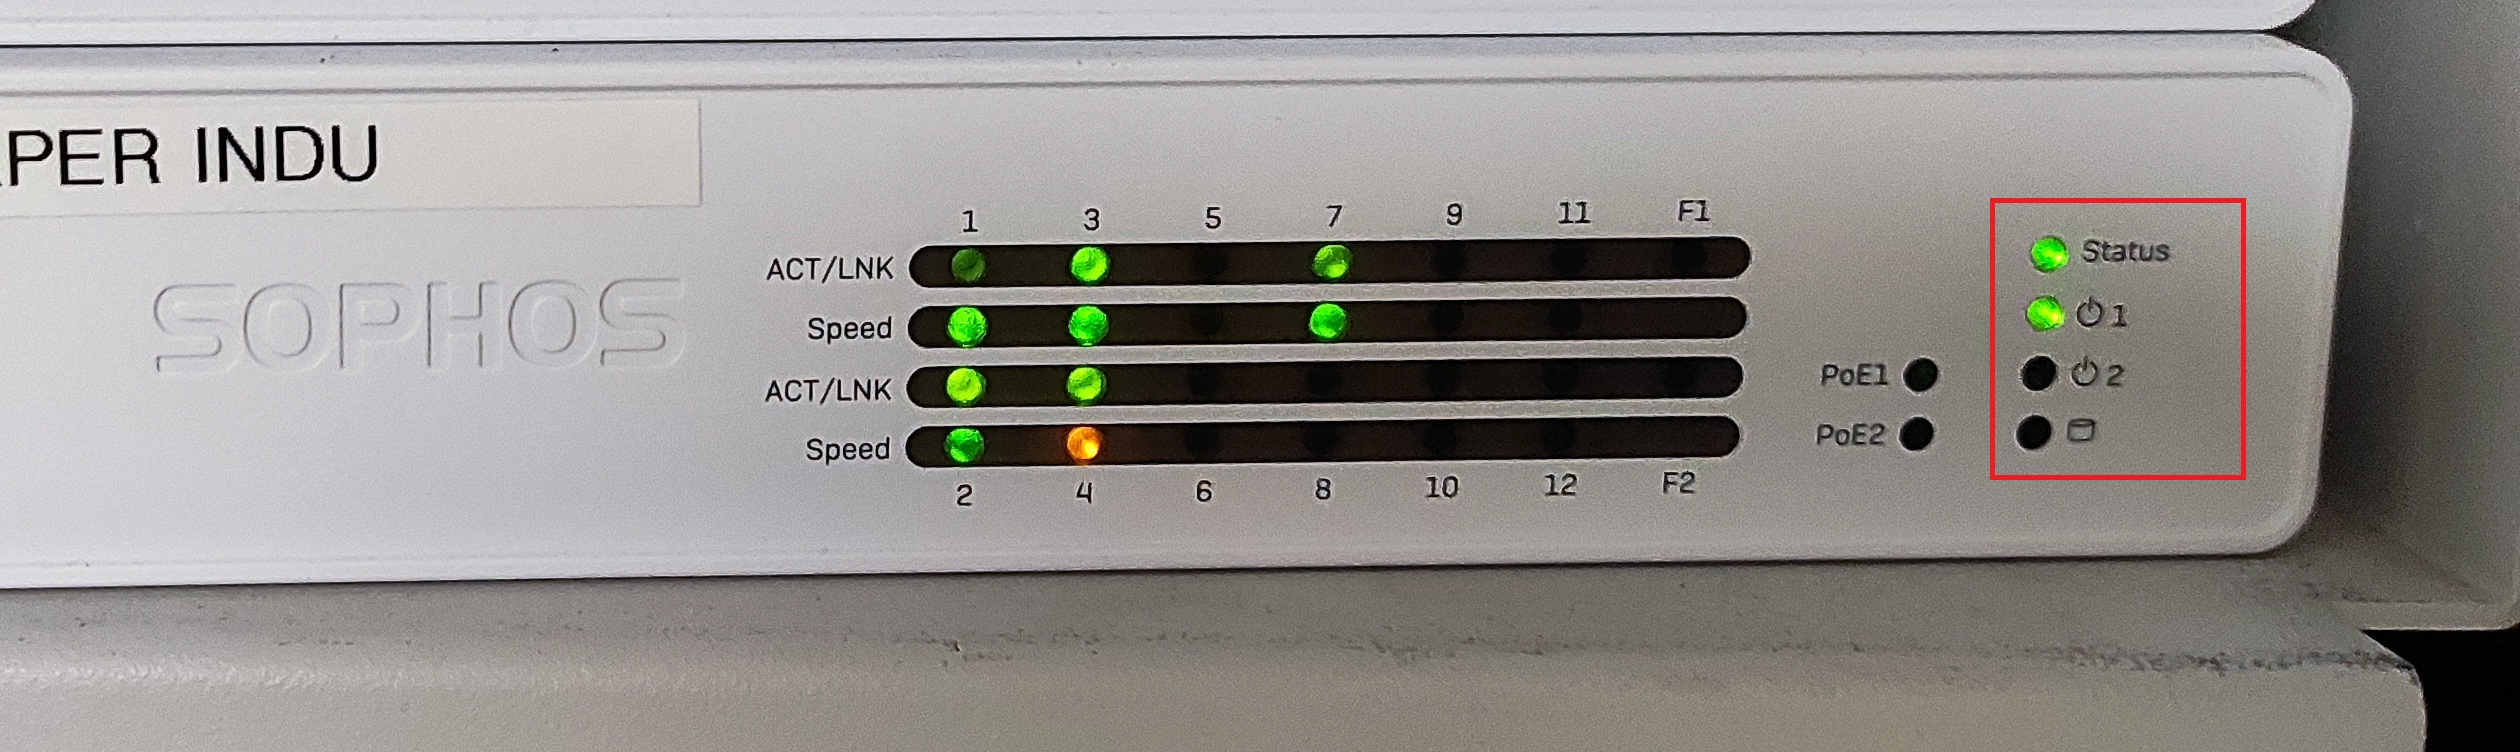
\includegraphics[width=0.8\textwidth]{fotos/SophosFirewall_LEDStatus.jpg}
    \caption[Sophos Firewall]{\label{fig:grail}Foto van dee huidige Sophos firewall die in gebruik is op de FR16 site van VPK. Uit de afbeelding blijkt dat beide firewalls slechts één externe voeding gebruiken en dat deze zich in normale werking bevinden.}
\end{figure} 



\subsection{Product should provide zero downtime software upgrades as configured in the HA environment}
Binnen deze criteria streeft VPK ernaar om de continuïteit van de productie te waarborgen tijdens het uitvoeren van firmware updates op de firewalls. Dit is om twee redenen van groot belang.
Enerzijds wil VPK garanderen dat de firewalls altijd voorzien zijn van de meest recente en ondersteunde firmwareversies. Regelmatige updates verminderen het risico op cyberaanvallen die misbruik maken van kwetsbaarheden in oudere firmware.
Anderzijds is het cruciaal dat de productieprocessen op de site ononderbroken blijven. Omdat vrijwel alle machines afhankelijk zijn van externe netwerkverbindingen, bijvoorbeeld voor communicatie met SAP-servers is een constante en veilige verbinding met de servers die buiten het netwerk liggen essentieel.

Om deze beschikbaarheid te garanderen, is het noodzakelijk dat de twee firewalls, die in een High Availability configuratie zijn opgesteld, zodanig worden geüpgraded dat altijd minstens één firewall actief blijft. Zo kan het netwerkverkeer tijdens de update veilig blijven verlopen, zonder impact op de productie.

\textbf{Sophos}
\begin{itemize}[label=\textbullet]
    \item Sophos biedt een snelle en eenvoudige manier aan om een HA firewall pair te upgraden zonder dat er downtime is. In HA zullen deze apparaten opereren als een enkele entiteit. Waarbij één van de apparaten zich zal voordoen als primaire firewall en de andere als back-up firewall. Omdat deze apparaten werken in een cluster is het aantal stappen dat moet worden genomen om deze apparaten te updaten eerder beperkt. De gebruiker zal zal op de GUI van de primaire sophos firewall slechts twee knoppen moeten indrukken om het upgrade process te starten. Eerst zal de user op de download knop moeten drukken om de nieuwe firmware te downloaden vanop het internet. Daarna zal de user op de install knop moeten drukken om de firmware effectief te installeren. De verdere processen die moeten worden uitgevoerd om de firewalls te upgraden gebeurt volledig automatisch op de achtergrond. Het process dat zich op de achtergrond plaatsvind verloopt als volgt:
    
    
    
    Sophos biedt een snelle en eenvoudige manier om een HA-firewallpair te upgraden zonder enige vorm van downtime. In een HA configuratie functioneren beide apparaten als één geheel, waarbij één toestel optreedt als de primaire firewall en het andere als de back-up, dit noemt men een cluster. Doordat deze apparaten in een cluster werken, is het aantal benodigde stappen die door de gebruiker moeten worden uitgevoerd om een upgrade uit te voeren beperkt.
    
    De gebruiker hoeft op de GUI van de primaire Sophos firewall slechts twee knoppen te gebruiken om het upgradeproces te starten. Eerst wordt op de download knop geklikt om de nieuwste firmware van het internet te downloaden. Vervolgens wordt met een druk op de install knop de installatie van de firmware gestart.
    
    De verdere stappen van het upgradeproces verlopen volledig automatisch op de achtergrond. Dit proces bestaat uit de volgende fasen:
    
    \begin{enumerate}
        \item Het primaire apparaat (apparaat A) voert een upgrade uit van het secundaire apparaat (apparaat B).
        \item Apparaat B start opnieuw op met de nieuwe firmware en neemt de controle over het netwerk over. Het wordt nu het primaire apparaat, terwijl apparaat A de rol van secundair opneemt.
        \item Apparaat A voert daarna zelf de upgrade naar de nieuwe firmware uit. Het blijft het secundaire apparaat, tenzij het oorspronkelijk als geprefereerde primaire is geconfigureerd — in dat geval zal het cluster automatisch terugschakelen.
    \end{enumerate}


\end{itemize}

\textbf{Palo Alto}
\begin{itemize}[label=\textbullet]
    \item Hoewel het upgraden van een Sophos HA-firewallpair via een eenvoudige methode verloopt die geen diepgaande kennis van High Availability vereist, is dit bij Palo Alto niet het geval. Palo Alto biedt namelijk geen mogelijkheid om firmware-upgrades automatisch uit te voeren via een automatische failover. Bij het upgraden van een Palo Alto-firewallpair moet op elk apparaat afzonderlijk de firmware handmatig worden gedownload en geïnstalleerd. Daarnaast moet de failover tussen de twee firewalls handmatig worden uitgevoerd. Deze manuele aanpak maakt het upgradeproces aanzienlijk complexer en tijdrovender in vergelijking met Sophos. 
    
    Toch is het uitvoeren van firmware upgrades een cruciale taak om de beveiliging van het netwerk up-to-date te houden. Indien de persoon die de upgrade uitvoert niet volledig op de hoogte is van de specifieke stappen en aandachtspunten bij een HA upgrade binnen Palo Alto, kunnen er snel fouten ontstaan. Zulke fouten kunnen leiden tot onverwachte downtime van de productieomgeving, met potentieel ernstige financiële gevolgen. Om dit risico te minimaliseren, zal er een PoC worden opgesteld. Deze PoC dient niet alleen om het upgradeproces vooraf te testen, maar zal ook fungeren als een gedetailleerde handleiding voor het veilig en gecontroleerd upgraden van een Palo Alto HA firewall pair binnen een productieomgeving.
\end{itemize}

\subsection{The product must support a minimum of 5 Million concurrent connections}
Deze eis specificeert dat de firewall minimaal 5 miljoen gelijktijdige sessies moet kunnen ondersteunen. Dit is van cruciaal belang om te waarborgen dat de netwerkcapaciteit ook tijdens pieken voldoende is. VPK wil hiermee voorkomen dat het aantal actieve sessies ooit een bottleneck vormt voor de netwerkprestaties of de beschikbaarheid van kritieke bedrijfsapplicaties. Dit criterium draagt dan ook direct bij aan de betrouwbaarheid en schaalbaarheid van de infrastructuur.

Het maximum aantal gelijktijdige sessies op de Palo Alto PA-440 firewall is: 200.000 \newline
Het maximum aantal gelijktijdige sessies op de Sophos XGS 136 firewall is: 6.400.000

\subsection{The product must support a minimum of 120.000 new connections per second processing.}
Deze vereiste stelt dat het systeem in staat moet zijn om minimaal 120.000 nieuwe sessies per seconde te verwerken. Dit is van belang om te garanderen dat de firewall adequaat kan omgaan met plotselinge pieken in netwerkverkeer, zoals tijdens geautomatiseerde processen of het opstarten van systemen. Deze specificatie is vooral belangrijk in dynamische omgevingen waar connectiviteit met externe servers die zich niet on-prem begeven te communiceren.

Het maximale nieuwe sessies per seconde van de Palo Alto PA-440 firewall is: 37.000 \newline
Het maximale nieuwe sessies per seconde van de Sophos XGS 136 firewall is: 74.500

\begin{table}[h!]
    \centering
    \resizebox{\textwidth}{!}{%
        \begin{tabular}{|l|l|l|}
            \hline
            \textbf{Device} & \textbf{Max Concurrent Sessions} & \textbf{New Connections per Second} \\
            \hline
            PA-440 & 200{,}000 & 37{,}000 \\
            XGS 136 & 6{,}400{,}000 & 73{,}000 \\
            Required & 5{,}000{,}000 & 120{,}000 \\
            \hline
        \end{tabular}%
    }
    \caption{Vergelijking van maximale gelijktijdige sessies en nieuwe verbindingen per seconde voor PA-440 en XGS 136 firewalls.}
\end{table}


\subsection{Product must have a central cloud management solution}


\textbf{Sophos}
\begin{itemize}[label=\textbullet]
    \item 
\end{itemize}

\textbf{Palo Alto}
\begin{itemize}[label=\textbullet]
    \item 
\end{itemize}


\subsection{Vergelijk van andere criteria van de RFP.}



\section{Sophos en Palo Alto licenties}
Naast het aankopen van de effectieve firewall moet men ook steeds rekening houden met de kosten voor het aankopen van de geschikte licenses. Palo Alto en Sophos maken beiden gebruik van een model waarbij ze
geavanceerde functionaliteiten samenvoegen in bundels die je dan nog apart dient aan te kopen. Zowel voor Sophos als voor Palo Alto moet je deze license jaarlijks vernieuwen.


\subsection{Sophos Licenties}
Bij Sophos XGS firewalls is de 'Base License' standaard en gratis inbegrepen. Deze license beschikt over een aantal essentiële basisfuncties, zonder dat een betaalde licentie nodig is. De licentie omvat onder andere een stateful firewall, die verkeer zal inspecteren en doorsturen. Een VPN-functionaliteit (zoals IPsec en SSL VPN) voor veilige externe toegang. Ook High Availability is inbegrepen, waarmee twee firewalls gekoppeld kunnen worden voor automatische failover bij een onverwachte storing.

Echter bied Sophos nog een aantal andere extra licenses aan iedere license en de beschikbare functionaliteiten worden hieronder in detail besproken:

\textbf{Network Protection}
\begin{itemize}[label=\textbullet]
    \item De network protection bundel van Sophos bevat een reeks netwerk gerelateerde beveiligingsfuncties. Zo bevat deze bundel onderandere een next geration IPS oplossing die data op applicatieniveau zal gaan blokeren. Ook zal er gebruikt kunnen worden gemaakt van de security heartbeat die een link creeren tussen de firewall en endpoints die verbonden zijn met Sophos Central, hierdoor zullen dreigingen sneller kunnen worden opgemerkt en kan de mogelijke impact beperkt blijven. Ook zal er een clientless HTML5 self-service portal beschikbaaar zijn waardoor gebruikers vooraf gedefinieerde bronnen remote zullen kunnen bereiken.
\end{itemize}

\textbf{Web Protection}
\begin{itemize}[label=\textbullet]
    \item De Web Protection bundel van Sophos zorgt voor uitgebreide controle over het internet en applicatiegebruik van de gebruikers binnen het netwerk. Er kunnen regels worden ingesteld per gebruiker of groep, zo kunnen bepaalde URL's worden geblokeerd op basis van zelfgekozen zoekwoorden. Met application control wordt inzicht verkregen in duizenden applicaties en kan worden bepaald wat wel of niet is toegestaan, hier kan er ook QoS worden ingesteld. Dankzij Synchronized Application Control worden onbekende applicaties automatisch herkend. De geoptimaliseerde SSL inspection zorgt ervoor dat ook geëncrypteerd verkeer gecontroleerd wordt, zonder de de snelheid hieronder lijd.
\end{itemize}

\textbf{Zero Day Protection}
\begin{itemize}[label=\textbullet]
    \item De Zero Day Protection bundel van Sophos biedt AI gebaseerde statische file analyse technieken aan die actief ransomware en andere onbekende dreigingen zullen neutraliseren. Een aantal verschillende functies die aanwezig zijn in deze bundel zijn: een cloud-based threat intelligence and threat analysis platform, dit platform zal aan de hand van deep learning gebaseerde analyse een 'Risk Summary' voor een file aanmaken. Ook is er statische file analyse inbegrepen, deze functie zal aan de hand van verschillende ML modellen dreigingen identificeren.
\end{itemize}

\textbf{DNS Protection}
\begin{itemize}[label=\textbullet]
    \item De DNS Protection bundel van Sophos biedt verschillende functies die gefocust zijn op het beschermen van de DNS. Deze bundel zal je onder andere toelaten om de cloud gebaseerde DNS service te gebruiken. Deze service zal in de eerste instantie werken als een standaard DNS server, maar zal er ook voor zorgen dat onveilige domeinen zullen worden geblokkeerd over het volledige netwerk. Dankzij SophosLabs zal de Sophos DNS Protection regelmatig worden geüpdatet om zo de nieuwste kwaadaardige en ongewenste websites te blokkeren.
\end{itemize}

\textbf{Central Orchestration}
\begin{itemize}[label=\textbullet]
    \item De Central Orchestration bundel van Sophos zal er voor zorgen dat meerdere Sophos firewalls met elkaar kunnen verbinden aan de hand van VPN verbindingen. Via deze license kan je ook op een eenvoudige manier verschillende complexe netwerk structuren opzetten, zoals mesh netwerken en hub-and-spoke netwerken.
\end{itemize}

\textbf{Email Protection}
\begin{itemize}[label=\textbullet]
    \item De Email Protection bundel van Sophos biedt een uitgebreide aantal functies voor het beveiligen van emailverkeer, zowel in de cloud via Sophos Central Email Advanced als lokaal via on-box implementatie. De bundel bevat verschillende functies zoals anti-spam, data loss prevention en emailencryptie. Dankzij de geïntegreerde message transfer agent wordt de continuiteit van de emails gegarandeerd, doordat de firewall automatisch berichten in een wachtrij plaatst wanneer mailservers onbereikbaar zijn. Met live anti-spam worden gebruikers beschermd tegen de nieuwste spamcampagnes, phishingaanvallen en schadelijke bijlagen. Daarnaast biedt Sophos met SPX een unieke, wachtwoordgebaseerde emailencryptieoplossing die ook werkt zonder bestaande trustinfrastructuur bij de ontvanger.
\end{itemize}

\textbf{Web Server Protection}
\begin{itemize}[label=\textbullet]
    \item  De Web Server Protection bundel van Sophos biedt uitgebreide beveiliging voor webservers. Deze bundel heeft als doel het netwerk te beschermen tegen hackingpogingen en tegelijkertijd veilige externe toegang mogelijk te maken. Dankzij vooraf gedefinieerde beleidsjablonen kunnen veelgebruikte toepassingen zoals MS Exchange en SharePoint snel en eenvoudig worden beveiligd. De bundel bevat ook geavanceerde beschermingstechnologieën zoals URL en formulierverharding, bescherming tegen deep-linking en directory traversal, evenals beveiliging tegen SQL-injecties, cross-site scripting en andere veelvoorkomende aanvallen. Ook zullen er geïntegreerde reverse proxy functionaliteiten zoals authenticatieopties, SSL offloading en load balancing aanwezig zijn. Hierdoor worden niet alleen de beveiliging maar ook de prestaties van publiek toegankelijke servers geoptimaliseerd.
\end{itemize}

\subsection{Sophos Licenties die nuttig kunnen zijn voor VPK.}
Sophos biedt een uitgebreid gamma aan licenties voor netwerkbeveiliging, gaande van bescherming tegen zero-day aanvallen tot e-mailbeveiliging. In theorie is het mogelijk om elk aspect van het VPK netwerk te beschermen door alle beschikbare Sophos-licenties aan te schaffen. Binnen de context van VPK is dit echter niet relevant. VPK maakt namelijk al gebruik van diverse gespecialiseerde services die functies vervullen waarvoor Sophos licenties aanbiedt. Het aankopen van bijkomende licenties zou in dat geval overbodig kunnen zijn. Daarom zullen alle beschikbare Sophos-licenties kritisch worden geanalyseerd om te beoordelen of ze daadwerkelijk toegevoegde waarde bieden voor de bestaande infrastructuur van VPK. Enkele bundels die een meerwaarde zouden kunnen bieden aan VPK worden in de volgende punten besproken.


\textbf{Network Protection bundel}

VPK beschikt momenteel niet over de mogelijkheid om IPS functionaliteiten centraal te beheren. De Network Protection licentie biedt ondersteuning voor de implementatie van IPS rechtstreeks binnen de firewall, wat essentieel is voor een snelle en efficiënte reactie op potentiële dreigingen van buitenaf. Om de integriteit en beschikbaarheid van het netwerk te waarborgen, is het cruciaal dat deze functie wordt ingeschakeld. Daarom kan worden geconcludeerd dat deze licentie een must is, mocht VPK besluiten om een Sophos firewall te implementeren.


\textbf{DNS Protection bundel}
De DNS Protection bundel voegt verschillende DNS gerelateerde beveiligingsfuncties toe aan de Sophos firewall. Binnen VPK wordt echter al gebruikgemaakt van een eigen DNS server waarop specifieke regels zijn toegepast. Hierdoor lijkt het overbodig om te investeren in een licentie die functionaliteiten biedt die VPK reeds centraal en voor alle sites heeft opgezet. Deze bundel zou daarentegen wel een waardevolle optie zijn in situaties waarin VPK geen eigen DNS server zou gebruiken. Bovendien biedt de Sophos oplossing aanvullende mogelijkheden die momenteel niet aanwezig zijn in de bestaande infrastructuur, zoals AI-gestuurde functies voor het in real-time blokkeren van kwaadaardige domeinen.


\textbf{Central Orchestration bundel}
VPK is aangesloten op het Proximus-netwerk en bevindt zich momenteel in de overgang van een MPLS omgeving naar een SD-WAN oplossing. De functies die deze licentie biedt, richten zich voornamelijk op het verbinden van verschillende vestigingen via VPN-technologie. Aangezien VPK al beschikt over een centrale netwerkarchitectuur die deze functionaliteiten afdekt, is het aanschaffen van deze licentie voor de Sophos-firewall in dit geval niet aanbevolen. De toegevoegde waarde zou beperkt zijn binnen de bestaande infrastructuur. Maar mocht VPK nog geen MPLS en SD-WAN omgeving hebben bij Proximus dan zou deze licentie wel zeer waardevol kunnen zijn omdat je op een eenvoudige manier zonder gebruikt te moeten maken van andere fysieke hardware of services centraal je volledige netwerkstructuur zou kunnen beheren.


\textbf{Email Protection bundel}
VPK maakt momenteel gebruik van de Cisco IronPort service voor het filteren en beveiligen van emailverkeer. Aangezien deze oplossing alle functionaliteiten dekt die ook door deze Sophos licentie worden aangeboden, is de aankopen van deze licentie niet aan te raden. De meerwaarde binnen de bestaande infrastructuur van VPK zou hierdoor minimaal zijn.


\textbf{Web Server Protection bundel}
WIP ik weet niet wat VPK voor web protection gebruikt.




\chapter{Configuratie van de firewall opstelling}
\label{ch:configFW}

Op basis van de verzamelde info en de huidige problemen op de productiesite van Alizay, lijkt het logisch om te kiezen voor één soort firewall die goed past bij de bestaande infrastructuur en kennis binnen VPK. Een overstap naar een Palo Alto firewall heeft op dat vlak verschillende voordelen.

Met deze oplossing kan het beheer van alle firewalls binnen VPK op één plek gebeuren. Dat maakt het dagelijkse werk minder ingewikkeld. Ook gebruiken andere VPK-sites al Palo Alto, wat zorgt voor meer eenheid. Zo kan er beter gebruik gemaakt worden van bestaande kennis, werkwijzen en tools. Dit zorgt voor een veiligere en efficiëntere werking van zowel IT- als OT-netwerken. Tegelijk verkleint het de kans op fouten of verkeerde instellingen.

Doordat Palo Alto al op meerdere plaatsen binnen VPK gebruikt wordt, kan het netwerkteam sneller reageren bij problemen of aanpassingen doen zonder hulp van buitenaf nodig te hebben. Aangezien het huidige OT-netwerk vrij complex is, is het ook belangrijk dat de firewall goede ondersteuning biedt voor het opdelen van het netwerk, het opvolgen van verkeer en het beheren van wie toegang heeft tot wat.

Daarom lijkt het logisch om de Sophos firewall te verwijderen uit het netwerk, en enkel gebruik te maken van een Palo Alto firewall pair.

\newpage

\section{Verzamelen en verwerken van Logs}

\subsection{Logs via Palo Alto}
De Palo Alto firewalls die zich op andere locaties bevinden, verzamelen loggegevens van netwerkverkeer en systeemactiviteiten. Deze logs worden automatisch doorgestuurd naar een centrale server waarop Microsoft Sentinel draait. Microsoft Sentinel is een cloudgebaseerde SIEM-oplossing van Microsoft. SIEM staat voor Security Information and Event Management.
Een SIEM systeem verzameld loggegevens uit verschillende bronnen, zoals firewalls, servers, toepassingen en andere netwerkapparaten. Die gegevens worden vervolgens geanalyseerd. Als er iets gebeurt dat afwijkt van het normale gedrag, kan Sentinel dit detecteren in realtime. Het systeem kan daarna automatisch meldingen sturen of zelfs actie ondernemen, zoals het blokkeren van een IP-adres of het starten van een onderzoek. Zo helpt Sentinel bij het vroegtijdig opsporen van cyberdreigingen en bij het verbeteren van de beveiliging van het netwerk.


Naast Microsoft Sentinel worden de verzamelde loggegevens ook doorgestuurd naar de Zabbix monitoringserver. Zabbix is een open-source monitoringtool die gebruikt wordt om IT-infrastructuur te bewaken. Dit omvat onder andere fysieke servers, virtuele machines, netwerksystemen en cloudtoepassingen.
Zabbix verzamelt allerlei metrics zoals CPU-belasting, geheugengebruik, schijfruimte, netwerkactiviteit, enzovoort. Deze informatie wordt weergegeven in een overzichtelijk dashboard dat je via een webinterface kan bekijken. Zo kan er in één oogopslag gezien worden of er problemen zijn met een bepaald systeem of apparaat.
Zabbix maakt het ook mogelijk om alerts te versturen wanneer bepaalde drempels worden overschreden, bijvoorbeeld als de CPU belasting te hoog is of als een server niet meer reageert. Op die manier kunnen problemen snel worden gedetecteerd en opgelost, voordat ze ernstige gevolgen hebben.

\begin{figure}[H]
    \centering
    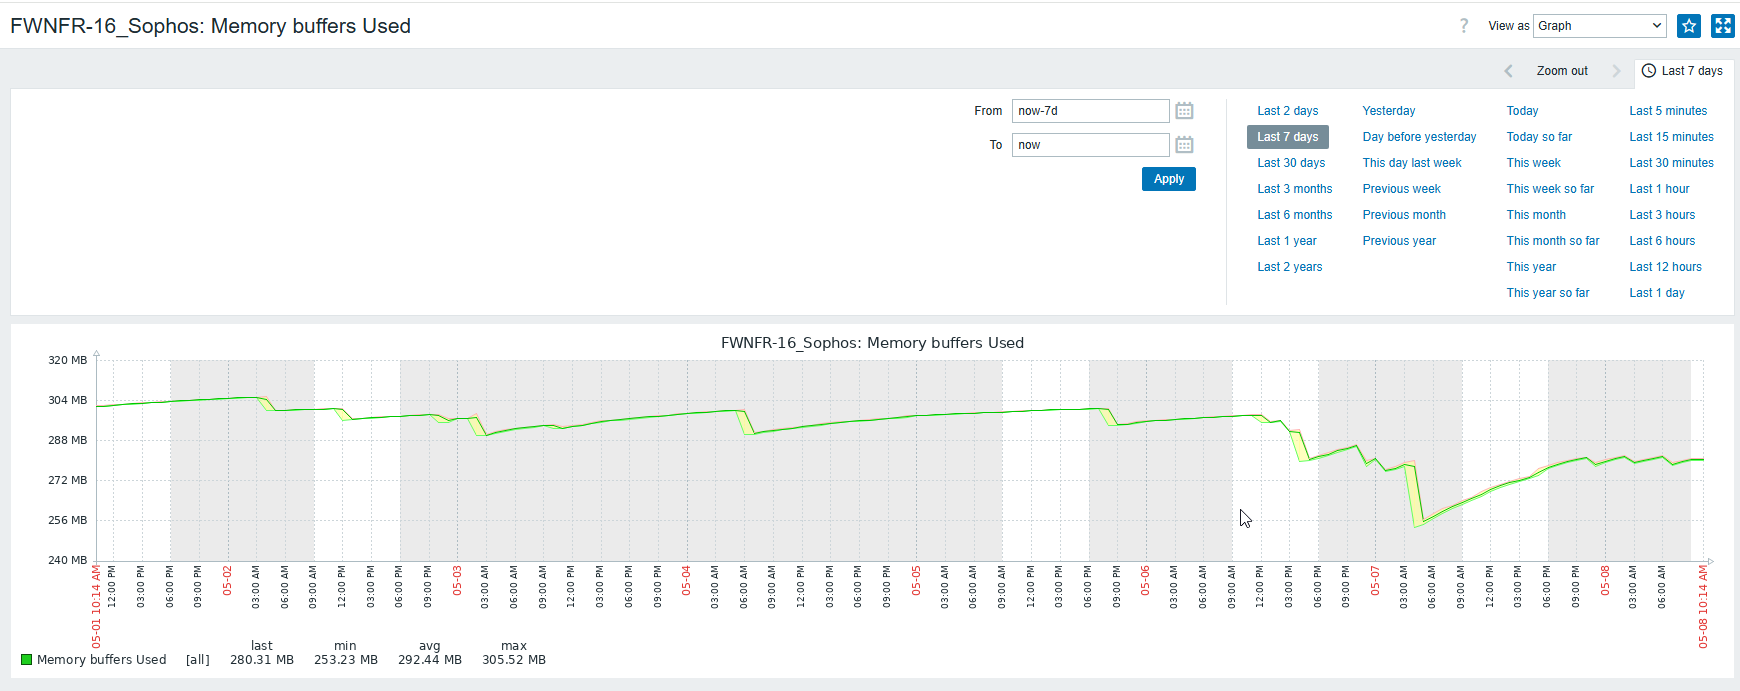
\includegraphics[width=0.9\textwidth]{fotos/SophosZabbix.png}
    \caption[Sophos Memory Buffer in Zabbix]{\label{fig:grail}Een grafiek uit Zabbix die het geheugengebruik van de memory buffers van de Sophos firewall in Mega Bytes weergeeft.}
\end{figure} 


\subsection{Logs via Sophos}
Tot voor kort werden er op de Sophos firewall geen loggegevens verzameld. Hierdoor was er weinig zicht op wat er zich precies afspeelde binnen het netwerkverkeer dat via deze firewall liep. Als onderdeel van mijn bachelorproef heb ik ervoor gezorgd dat de firewall nu wel logs verzamelt en dat deze op een correcte en veilige manier worden doorgestuurd naar de nodige servers die de data analyseren en verwerken.
De loggegevens worden via het syslog-protocol doorgestuurd naar twee verschillende servers: enerzijds de Zabbix monitoringserver en anderzijds de Microsoft Sentinel server. Deze syslog-berichten bevatten nuttige informatie, zoals de actuele firewallregels, de heartbeat van het systeem en verschillende systeemgebeurtenissen.
Omdat er op het FR16-netwerk tot nu toe nauwelijks of geen monitoring aanwezig was, is deze wijziging van groot belang. Dankzij deze aanpassing kunnen problemen sneller worden opgemerkt. In het geval van downtime of een mogelijke cyberdreiging kan er sneller worden ingegrepen, wat uiteindelijk helpt om schade of downtime te beperken.



\section{Beste High Availability settings voor de Palo Alto firewalls van FR16.}


High Availability (HA) is een functie die verschillende netwerk apparatuur vendors aanbieden, deze functie zorgt ervoor dat de downtime geminimaliseerd wordt door het gebruiken van meerdere entiteiten van dezelfde appartuur. Vaak zal er gebruik worden gemaakt van twee apparaten die dan op verschillende mogelijke manieren geconfigureerd kunnen worden. Twee populaire manieren om deze apparaten te configurenen zijn Active/Active of Active/Passive. De termen Active en Passive slaan hier op de staat van het apparaat. Active betekend dat dit apparaat wel degelijk bepaalde netwerk functies op zich zal nemen en dus actief zal meerwerken om bepaalde data te verwerken. Passive betekend dat het apparaat niet actief data zal verwerken, en zich dus in een soort van rust stand bevindt.

\subsection{Active/Active firewall opstelling}
Bij een Active/Active opstelling verwerken beide apparaten actief data. In dit geval zullen beide firewalls gelijktijdig verkeer filteren op basis van vooraf gedefinieerde firewallregels. Hoewel dit in sommige situaties voordelen kan bieden, is deze opstelling in onze omgeving minder geschikt om meerdere redenen.
\newline



\begin{itemize}
    \item \textbf{Active/Active firewall pairs zijn complex om te installeren en onderhouden:}  Sessie synchronisatie tussen de firewalls kan complex worden, zeker als er gebruik wordt gemaakt van dynamische IP’s binnen het netwerk. Omdat er is besloten in bovenstaande rasci matrix dat het beheer van de OT firewall een verantwoorddelijkheid is van het OT team lijkt het niet verstandig om gebruik te maken van een complexe firewall opstelling omdat de kennis over het beheer van dit soort opstellingen minder groot is bij het OT team. 
    
    \item \textbf{Kans op asymmetrische sessies:} De kans is groter dat beide firewalls onafhankelijk data forwarden, waardoor inbound verkeer via een ander pad kan terugkeren dan outbound verkeer. Dit kan leiden tot session mismatches, met als gevolg dat data mogelijk wordt gedropt.
    
    \item \textbf{Inconsistentie met andere sites:}  Alle andere VPK-sites met een Palo Alto firewall-pair gebruiken een Active/Passive-opstelling. Een Active/Active-configuratie binnen FR16 zou de uniformiteit van de netwerkarchitectuur verstoren.

\end{itemize}

\newpage

Ook is binnen deze Active/Active opstelling de mogelijkheid om gebruik te maken van parallel processing. Dit zorgt er effectief voor dat throughput verdubbeld wordt. \autocite{Fulp2006} Voor onze use case is dit echter niet relevant. De hoeveelheid data die via de Sophos firewall wordt verstuurd, is zo laag dat één Palo Alto firewall ruim voldoende capaciteit heeft om deze load zonder merkbare vertraging te verwerken. Uit een uitgebreide analyse van het netwerkverkeer op de WAN poort van de Sophos firewall, uitgevoerd over meerdere weken en op verschillende tijdstippen, blijkt dat de maximale gemeten throughput slechts 10 KBps bedroeg.


De nieuwe Palo Alto firewall (PA-440) zou een maximale throughput van 2,6 Gbps hebben en ondersteunt 200.000 gelijktijdige sessies. \autocite{PaloAltoDS2025} Dit betekent dat de beschikbare capaciteit ruimschoots volstaat en dat een Active/Active configuratie geen toegevoegde waarde biedt voor deze specifieke productiesite.

\begin{figure}[H]
    \centering
    \fbox{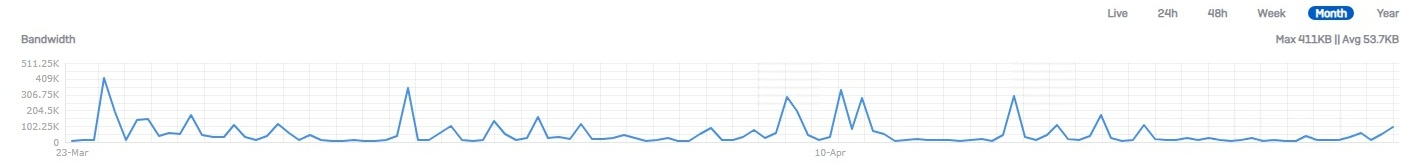
\includegraphics[scale=0.41]{fotos/SophosBandWidth.jpg}}
    \caption[Sophos firewall bandwidth graph]{\label{fig:grail}Totale bandbreedte die gebruikt wordt door de Sophos OT firewall van de productiesite van FR16}
\end{figure}




\subsection{Active/Passive firewall opstelling}

In een Active/Passive-opstelling is er slechts één firewall die gelijktijdig data verwerkt. Dit wordt mogelijk gemaakt door het configureren van HA-links. Deze links zijn cruciaal voor het waarborgen van redundantie, hoge prestaties en synchronisatie tussen firewalls in een HA-pair. Ze stellen de firewalls in staat om met elkaar te communiceren en statusinformatie te delen. Hierdoor kan de passieve firewall moeiteloos de taak van de actieve firewall overnemen bij een eventuele uitval. Zo zorgt de actieve firewall ervoor dat sessie-informatie wordt gedeeld met de passieve firewall, zodat deze altijd over de benodigde sessiegegevens beschikt in het geval van een failover. \autocite{PaloAltoHA2025} \autocite{PaloAltoHAb2025}

Verder in dit hoofdstuk zal een HA verbinding tussen twee firewalls worden geconfigureerd op basis van de behoeften van VPK en de algemene best practices.

\begin{figure}[H]
    \centering
    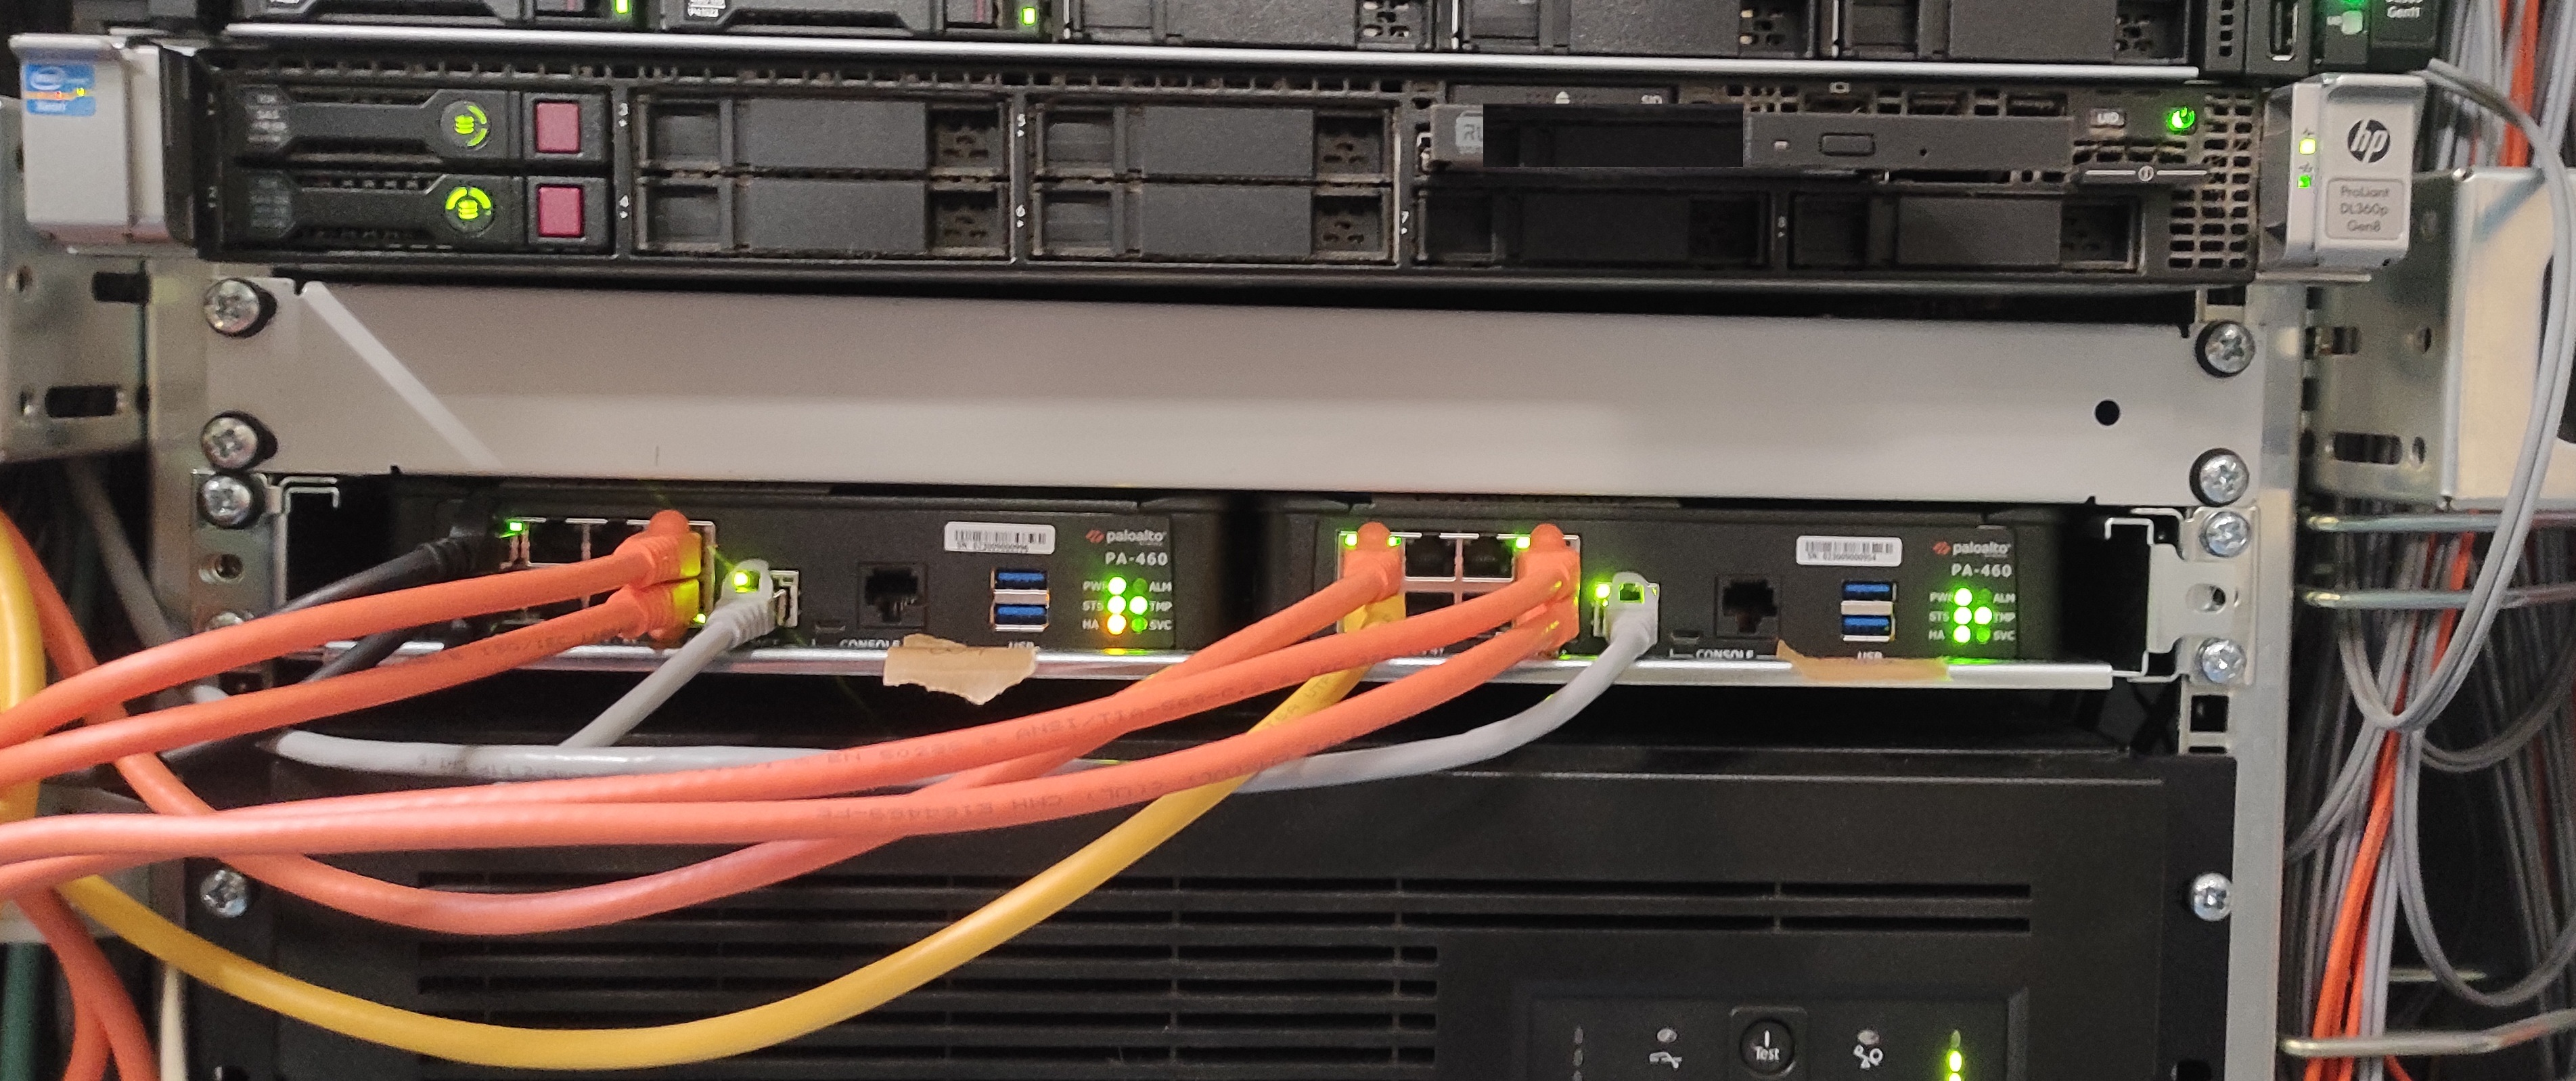
\includegraphics[width=0.8\textwidth]{fotos/PA_FirewallPairBE02.jpg}
    \caption[Palo Alto Active/Passive pair]{\label{fig:grail}Een Palo Alto Active/Passive firewall opstelling in de VPK site van Erembodegem.}
\end{figure} 



\section{Beste High Availability settings voor de Sophos firewall van FR16}

Om gebruik te kunnen maken van de HA-functies van de Sophos firewall is het noodzakelijk om twee identieke firewalls aan te schaffen. Momenteel is er echter slechts één firewall aanwezig, waardoor VPK genoodzaakt zal zijn om een tweede Sophos firewall aan te kopen om HA te kunnen implementeren. Dit proces is echter niet eenvoudig, aangezien het onduidelijk is hoe de huidige Sophos firewall is geconfigureerd. Als de twee firewalls in het HA-paar verschillende instellingen hebben, kan dit in de toekomst mogelijk problemen veroorzaken. Daarom moet er een tweede identieke firewall worden aangeschaft, en is het essentieel om een onderzoek te doen naar de huidige configuratie van de Sophos firewall.






\section{Configuratie van HA op een Palo Alto Firewall}

\textbf{Mode}
    \begin{itemize}[label=\textbullet]
        \item Zoals eerder in dit hoofdstuk besproken is zal er bij de configuratie van een Palo Alto firewall pair binnen een VPK site gebruik worden gemaakt van een Active/Passive opstelling. Hierbij zal er steeds slechts één firewall tegelijk actief zijn.
    \end{itemize}



\textbf{Enable Config Sync}
    \begin{itemize}[label=\textbullet]
        \item Configuration synchronization is een setting binnen Palo Alto HA firewall pairs. Waarbij een groot aantal settings automatisch worden gesyncroniseerd tussen devices. Om conflicten in configuraties te vermijden is het steeds aangeraden om configuraties steeds op de Active firewall uit te voeren en te wachten tot de Passive firewall gesynced is. Een aantal settings die niet worden gesynchroniseerd zijn: content updates, HA settings, mgmt interface settings, \ldots 
    \end{itemize}



\textbf{Passive Link state}
    \begin{itemize}[label=\textbullet]
        \item Deze settings zal bepalen in welke status alle data interfaces van een Passive firewall zullen worden geplaatst. Bij het gebruiken van de `shutdown` modus zullen alle data interfaces op de passive firewall in een `down` state worden geplaatst. Naast deze modus is er ook de `auto` modus. Bij deze modus zal alle data interfaces op `up` laten staan, maar dropped alle packets die over deze interfaces zouden passeren. Echter zou dit er voor kunnen zorgen dat switches nog steeds data packets zouden versturen over deze schijnbare `up` interfaces. Dit probleem samen met de algemene beste hardening cybersecurity practices om alle poorten die niet gebruikt worden op `down` te zetten zorgt ervoor dat VPK gebruik zal maken van de `shutdown` modus op beide firewalls.
    \end{itemize}



\textbf{Monitor fail hold down time}
    \begin{itemize}[label=\textbullet]
        \item De ``monitor fail hold down time'' is een vooraf ingestelde timer om onnodige failover te voorkomen. Nadat één van de links down gaat zal het process geen nieuwe failover toestaan als het ziet dat er binnen de tijdslimiet van één minuut de interface terug `up` is. Mocht de link toch langer dan één minuut down zijn zal er toch een failover gebeuren. Binnen iedere andere firewall op een VPK site wordt deze zelfde timer gebruikt. Daarom is er in het belang van uniformiteit gekozen om ook op deze site de timer in te stellen op één minuut.
    \end{itemize}



\textbf{Device Priority}
    \begin{itemize}[label=\textbullet]
        \item Deze settings zal bepalen welke prioriteit een bepaalde firewall heeft binnen een HA firewall pair. Een hogere waarde betekent direct ook een hogere prioriteit. Echter is dit enkel nuttig als men gebruik maakt van preemption. Maar aangezien preemption uit staat op deze firewalls zal deze priority waarde dus geen nut hebben.
    \end{itemize}



\textbf{Preemptive}
    \begin{itemize}[label=\textbullet]
        \item Deze setting zal er voor zorgen dat de firewall met een hogere prioriteit in staat is om terug Active te worden nadat er een failover is gebeurd. Echter heeft VPK gekozen om deze setting niet in te schakelen bij alle firewalls op alle VPK sites.
    \end{itemize}



\textbf{Hearbeat backup}
    \begin{itemize}[label=\textbullet]
        \item Deze optie zorgt ervoor dat er een backup is om de hearbeat berichten van de apparaten op te sturen via de management interfaces van de firewall. Deze berichten zullen standaard over de HA1 en HA2 link worden verstuurd. Aangezien er twee rechtstreekse linken zijn tussen de twee firewalls in het HA pair is het dus niet meer nodig om deze optie aan te zetten.
    \end{itemize}


\begin{figure}[H]
    \centering
    \fbox{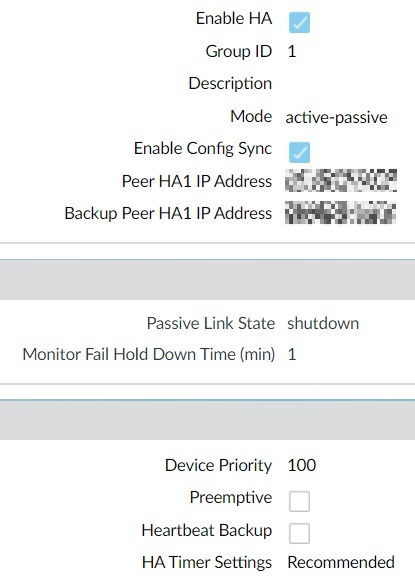
\includegraphics[scale=0.666]{fotos/PA_HASettings.jpg}}
    \caption[PA High Availability settings]{\label{fig:grail}GUI (Graphical User Interface) interface om de settings om de configuratie van High Availability op een PA firewall aan te passen.}
\end{figure}





\chapter{Opbouw firewallrules FR16}

\section{Firewallrules op Sophos}
\subsection{Manier voor het definieren van regels op Sophos}
\subsection{Specifieke regels van de Sophos firewall in FR16}

\section{Firewallrules op Palo Alto}
\subsection{Manier voor het definieren van regels op Palo Alto}
\subsection{Specifieke regels van de Palo Alto firewall in FR16}

\section{Netwerksegmentatie aan de hand van VLAN’s}

Netwerksegmentatie met VLAN’s (Virtual Local Area Networks) is nog steeds een erg goede manier om verschillende delen van een netwerk virtueel van elkaar te scheiden. Daarom lijkt het een slim idee om deze techniek ook toe te passen op het VPK-netwerk.

Concreet kan ervoor gekozen worden om de apparaten die binnen het IT/OT netwerk actief zijn onder te verdelen in verschillende groepen. Zo worden deze groepen van elkaar afgescheiden en is communicatie tussen hen standaard niet meer mogelijk. Uiteraard kunnen we nog steeds toestaan dat bepaalde groepen met elkaar praten via firewallregels op de Palo Alto firewall.

Het belangrijkste doel hiervan is simpel: als een aanvaller erin slaagt om toegang te krijgen tot één apparaat, dan krijgt hij niet meteen toegang tot het volledige netwerk, maar blijft hij beperkt tot het VLAN waarin dat toestel zich bevindt.

Om het allemaal overzichtelijk te houden, is het ook aangeraden om de VLAN’s te koppelen aan specifieke IP-ranges. Zo is het makkelijker om snel te zien in welk VLAN een bepaald toestel zit.

\subsection*{Voorbeeld VLAN-indeling}

\begin{table}[h!]
    \centering
    \begin{tabular}{|l|l|c|l|l|c|}
        \hline
        \textbf{DHCP} & \textbf{Usable range} & \textbf{VLAN} & \textbf{Name} & \textbf{Gateway} & \textbf{Mask} \\
        \hline
        10.x.2.0 & 10.x.2.1 -- 10.x.2.240 & 2 & AP mgmt & 10.x.2.254 & /24 \\
        10.x.4.0 & 10.x.4.1 -- 10.x.4.240 & 4 & Switch mgmt & 10.x.4.254 & /24 \\
        10.x.8.0 & 10.x.8.1 -- 10.x.8.240 & 8 & Server & 10.x.8.254 & /24 \\
        10.x.9.0 & 10.x.9.1 -- 10.x.9.240 & 9 & RF\_Corporate & 10.x.9.254 & /24 \\
        \hline
    \end{tabular}
    \caption{Een aantal gebruikte VLAN's binnen het VPK netwerk en bijhorende IP-ranges}
\end{table}

Uit het bovenstaande voorbeeld kan je afleiden dat er gekozen is om binnen VPK VLAN 8 te gebruiken voor alle servers binnen het netwerk. Zo weten we meteen dat een toestel met een IP-adres in de vorm van x.x.8.x een server is. Deze manier van werken brengt verschillende voordelen met zich mee:

\begin{itemize}
    \item \textbf{Overzichtelijkheid:} Door vaste IP-ranges per VLAN te gebruiken, is het snel duidelijk tot welke categorie een toestel behoort. Dit maakt het beheer en de troubleshooting veel eenvoudiger.
    \item \textbf{Beter beveiligd:} Apparaten die tot dezelfde functie horen (zoals servers) zitten samen in één VLAN. Dit beperkt de schade als er iets misloopt.
    \item \textbf{Efficiëntere netwerkconfiguratie:} Firewalls en andere beveiligingsregels kunnen veel gerichter ingesteld worden.
    \item \textbf{Makkelijker uitbreidbaar:} Je weet meteen in welke IP-range nieuwe toestellen moeten komen.
    \item \textbf{Snellere probleemoplossing:} Het IP-adres geeft snel inzicht in het type toestel en het netwerksegment.
    \item \textbf{Uniformiteit over verschillende sites:} Eén consistente VLAN-structuur vergemakkelijkt het beheer over meerdere locaties.
\end{itemize}

In het netwerk kan er ook voor gekozen worden om elke externe leverancier in een aparte VLAN onder te brengen. Bijvoorbeeld: Minda, Ducker, Bobst en Gopfert hebben elk hun eigen VLAN en aparte IP-range. Dit biedt heel wat voordelen:

\begin{itemize}
    \item \textbf{Verhoogde veiligheid:} Problemen blijven beperkt tot de VLAN van de leverancier.
    \item \textbf{Gerichte toegangscontrole:} Per VLAN kan je precies bepalen welke toegang een leverancier krijgt.
    \item \textbf{Compliance:} Helpt bij het voldoen aan interne en externe auditvereisten.
\end{itemize}

\section{Verschillende fases bij het deployen van firewall rules}

Bij de implementatie van de nieuwe firewalls wordt er gekozen om de firewallregels gefaseerd uit te rollen. Dit betekent dat niet alle regels in één keer actief worden, maar dat het netwerk stap voor stap verder wordt afgeschermd. Door steeds specifiekere regels in te voeren.

\subsection*{Voordelen van gefaseerde implementatie}

\begin{itemize}
    \item \textbf{Minder risico:} Fouten worden sneller opgemerkt en bijgestuurd.
    \item \textbf{Eenvoudigere probleemoplossing:} Door de gefaseerde aanpak kan men sneller de oorzaak van problemen vinden.
    \item \textbf{Beperkte OT documentatie:} Onverwachte sessies kunnen zonder onmiddellijke blokkering worden geanalyseerd.
    \item \textbf{Minimale impact op bedrijfsprocessen:} Kritieke toepassingen blijven beschikbaar tot in de laatste fase.
\end{itemize}

